\chapter{Joint Object Class Sequencing and Trajectory Triangulation (JOST)} \label{ch:jost}

\section{Introduction}

Techniques of 3D reconstruction from crowd-souced imagery have developped rapidly over the past decades, enabling systems to build 3D models from millions of images \cite{agarwal2011building,Frahm2010,zheng2014patchmatch,Heinly}. 
Despite these advances, the state-of-the-art methods only reconstruct the static part of a scene, but fail on the dynamic part. 
Since dynamic objects are typically the major focus of real-life images, it is of great interest to recover the 3D information of the dynamic objects to enable further applications.

%As the dynamic objects are typically the main focus of imagery, there is an demanding request 
%The main reason is that in typical datasets there is only a single view of any dynamic object, which impedes these methods from valid 3D triangulation.
%Hence, current techniques are not able to determine the 3D position of such objects. 
%This situation is regarded to have a highly limited potential for reconstruction as stated by \citet{Park_ECCV2010} and \citet{Valmadre_CVPR2012}.
In this work, we propose a method to estimate the 3D positions of dynamic objects of the same class moving in a common path from temporally uncorrelated images, \eg~a set of images capturing pedestrians walking on the sidewalk (see Figure \ref{fig:franklin_imgs}). 
The main challenge of the problem resides in the non-current captures of the dynamic objects, which invalidates the traditional 3D triangulation. 
Moreover, each instance of the object is typically observed by only one image and the temporal information across images is unknown. The only constraint available for our problem is the fact that all observed instances of an object class move along a common compact path in the 3D scene, which we define as an object class trajectory. For example, all the pedestrian instances walking on the sidewalk form an object class trajectory.

To attain the object class trajectory, our method simultaneously determines the sequence of the objects along the 3D path and the 3D positions of the objects on the path. Accordingly, this can be deemed as a joint object class equencing and trajectory triangulation, which generalizes the well known sequencing problem \cite{Basha_ECCV2012,Basha_ICCV2013} and the trajectory triangulation problem \cite{Valmadre_CVPR2012,ZhuCL_CVPR11,Park_ECCV2010} into a common framework. We leverage all the observations on different images to recover the object class trajectory, which then gives us the 3D positions of the dynamic objects.

%We formulate our problem as a non-convex optimization problem, and develop a novel solver comprising a step of discrete optimization followed by another step of continuous optimization. 
%The discrete step  a K-partite graph

%In fact, our proposed framework handles both of these problems as special cases. 
%The reconstructed object class trajectory then allows us to solve the generally ill-posed 3D reconstruction of a dynamic object from a single image by constraining the reconstruction on the 3D path of the object class. 
%An example of a single view reconstruction of two pedestrians is shown in Figure \ref{fig:FranklinSingleViewRecon}. %visualizing a generic person at the correct 3D position in the reconstruction of the 3D scene.

\begin{figure}[t]
\centering
\subfloat[]{
\centering
    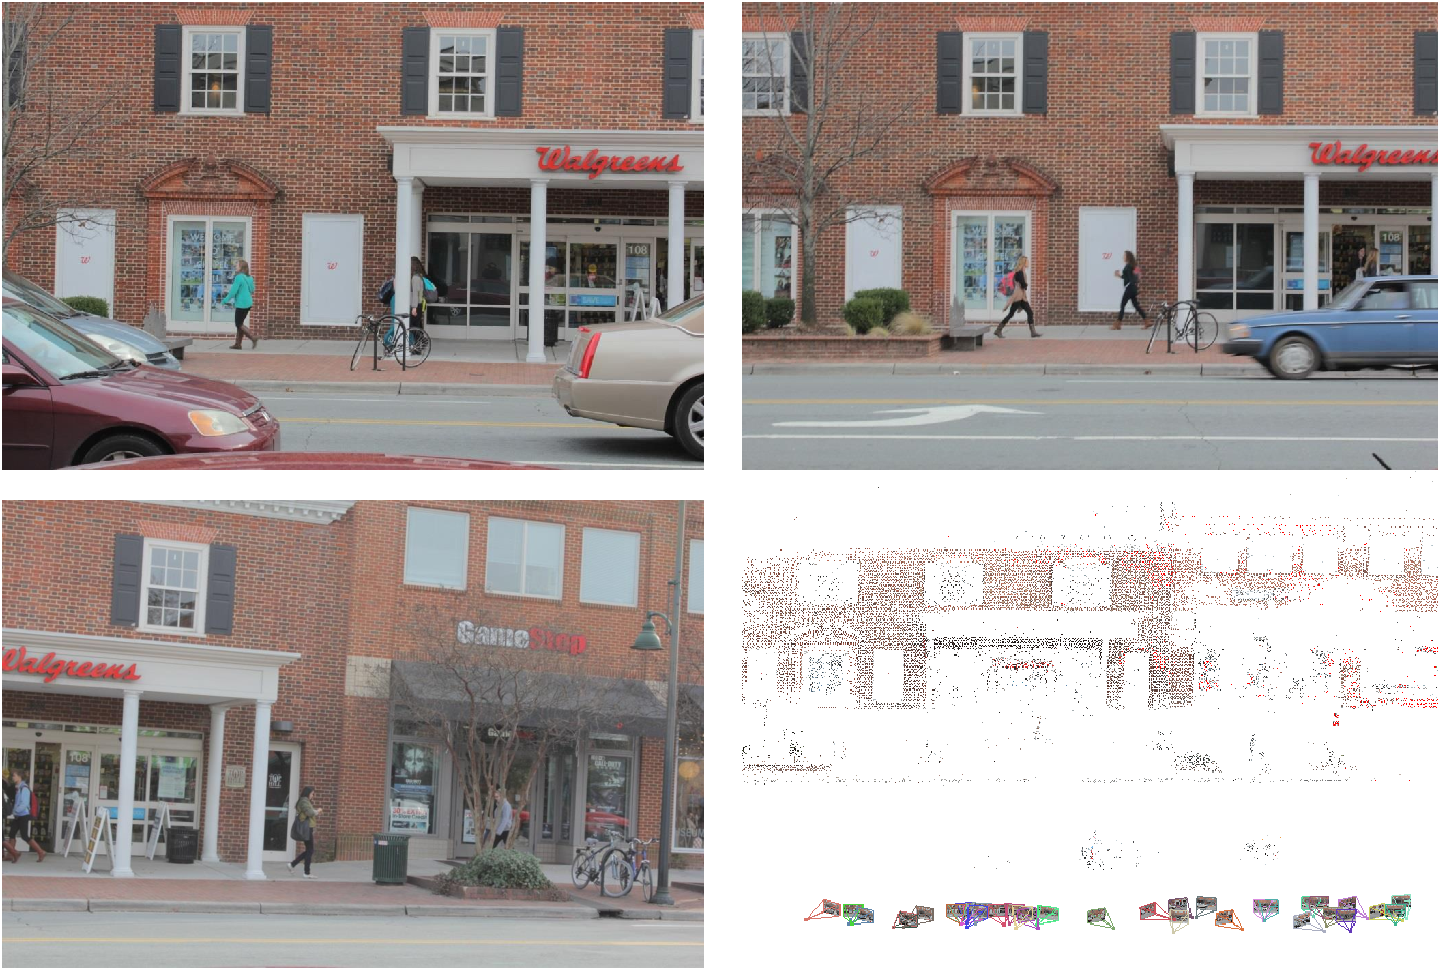
\includegraphics[height=0.34\linewidth]{chapter4/resource/images_cropped.pdf}
    \label{fig:franklin_imgs}
     \label{fig:franklin_sfm}
    }
\subfloat[]{
\centering
    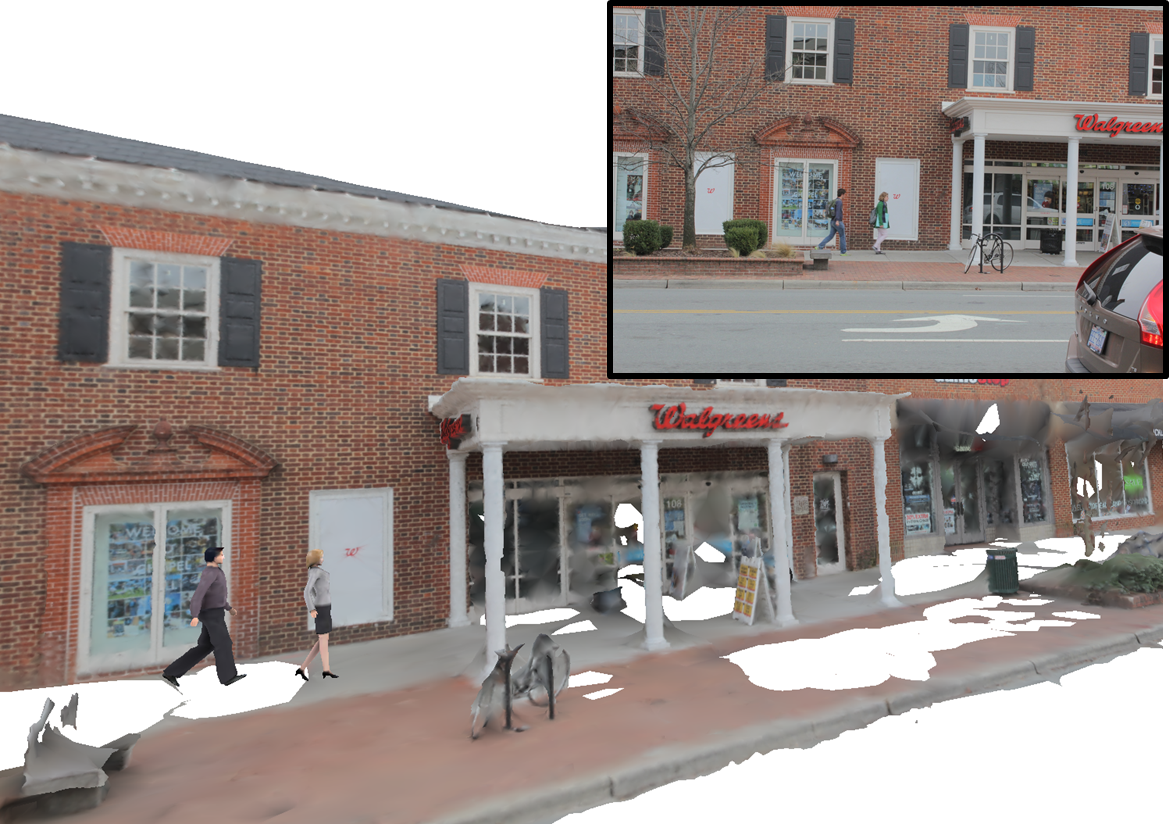
\includegraphics[height=0.34\linewidth]{chapter4/resource/3DModel.png}
    \label{fig:FranklinSingleViewRecon}
    }
\caption{Left: 3 images of the pedestrian dataset and the output of SFM. Right: The reconstruction of two pedestrians that are captured in the single image. Note we only reconstruction one 3D position for each dynamic object instance. For visualization purposes, a general mesh model is inserted into each estimated position.}
%\end{subfigure}
\label{fig:gmst}
\vspace*{-0.5cm}
\end{figure}

\section{\JOST}

We now detail our method for \jost~from uncontrolled image captures, which in particular removes the constraint of known temporal camera information and known object positions. To perform \jost~from the uncontrolled image set, we proceed as follows
\begin{enumerate}
\item \label{challenges_sfm} Spatially register the cameras to a common 3D coordinate system.
\item \label{challenges_tang} Detect object instances and estimate motion tangents from input imagery.
\item \label{challenges_order} Leverage the image positions of the object instances to simultaneously
\begin{enumerate}
\item Determine a camera ordering compliant with a continuous motion of the objects along a trajectory.
\item Triangulate the geometry of the corresponding motion path.
\end{enumerate}

\end{enumerate}
While we exploit known methods to solve for camera registration, object detection and motion tangents in the images, our main contribution is an algorithm for tackling challenge  \ref{challenges_order}. To tackle this challenge, we model our problem as a non-convex optimization problem, and develop a novel solver comprising a step of discrete optimization followed by another step of continuous optimization. 
Next, we introduce each step in detail.

\subsection{Spatial Registration}
The goal of the initial spatial registration in our method is to establish camera registration in a common coordinate system.
%There exists a large body of possible registration methods in structure from motion that can be used to register the cameras into a common coordinate system.
Given that in all our datasets a fair portion of the images contains static background structure, we use the publicly available structure from motion tool VisualSFM by Wu~\cite{WuVSFM}. It produces the camera registration and the sparse 3D points of the static structure. See Figure \ref{fig:franklin_sfm} for an example.

The obtained camera registration determines the camera center $\mathbf{\tilde{C}}_j$ of the $j$-th camera. In the paper we use bold font letters ${\mathbf x}$ to indicate that an entity is a vector and regular letters $x$ for scalar values. With the known camera calibration and registration, each pixel in the camera defines a ray direction $\mathbf{r}$ in the 3D scene  space. For our object class trajectory, we are only interested in the ray directions $\mathbf r_i$ for the different object $i$  of the desired class (for simplicity we refer in the paper to them as objects) with  $i =1, \dots, N$, where $N$ is the number of detected object class instances  over all frames. Hence, we only aim to compute the ray directions $\mathbf{r}_i$ for pixels belonging to the different detected objects $i$. The ray $\mathbf{X}_i$ in the 3D space represents a 1D subspace on which the imaged object has to lie and is described by:
\begin{equation}
\label{eq:ray}
\mathbf{X}_i(t_i)=\mathbf{C}_i + t_i \cdot \mathbf{r_i},
\end{equation}
where $t_i \geq 0$ is the positive distance from the camera center $\mathbf{C}_i$ along the ray $\mathbf{X}_i$.
In the remaining of the paper, we keep the condition $t_i \geq 0$ implicit for the purpose of concise formulation.
We denote the camera centers as $\mathbf{C}_i$  with $\mathbf{C}_i =\mathbf{\tilde{C}}_j$, where $\mathbf{C}_i$ is the center of the camera $j$ in which the object instance $i$ is detected. Please note that if more than one object is detected in camera $j$, there will be multiple $\mathbf{C}_i$ with identical positions. The unknown true distance of the object instance $i$ along ray $\mathbf{X}_i$ is denoted as $\hat{t}_i$. Once obtained, it determines the 3D object position $\mathbf{\hat{X}}_i$. %Next we turn to detail our object class instance detection and the motion tangent estimation.


\subsection{Object Detection and Motion Tangent Estimation}
\label{sec:detection}
Our proposed joint object class sequencing and trajectory triangulation leverages the motion tangent of the object instances, which is defined as the moving direction of the dynamic object in the 3D space. In this work, both object detection and motion tangent estimation are performed based on a single image.
For trajectory triangulation this has historically been solved by using videos for estimating the motion tangents~\cite{zhao2003face}, but for our proposed \jost~problem, temporal coherence or temporal proximity of the images cannot be assumed. Hence only motion tangent estimation based on a single image is applied.
The particular choice of object and motion tangent estimation method depends on the specific object class and the scenes.
We discuss our particular choices in Section \ref{sec:face_detection}, and for now we assume available the positions on each image defining the rays $\mathbf{X}_i$ and a coarse estimate of the motion tangent $\mathbf{d}_i$ of object $i$.
%quantized every $\theta^{\circ}$ between $-90^{\circ}$ and $90^{\circ}$. 
%In the following 
We determine the 2D position of each detected object $i=1,\dots, N$ on the image by the center of the bounding box.
%i.e. if the object is determined to be present in a connected component of the image, we represent its position through the center of gravity of that region.
%This simplifies the object class trajectories to the trajectory of a single characteristic object point. While in general this has the potential of slightly disturbing the trajectory, we empirically found that does not introduce any significant disturbance.
These object detections provide us a ray $\mathbf{X}_i(t_i)$ for each object observed in a camera, with the ray describing the one-dimensional subspace in which the detected object can be placed in the 3D space.
%Next %we will describe how the rays $\mathbf{X}_i(t_i)$ and the motion tangents of
%the objects are leveraged to compute the object class trajectory.


\subsection{Object Class Trajectory Estimation Problem}
\label{sec:problem}
%piecewise linear represented continuously or discrete
Assuming known rays $\mathbf{X}_i(t_i)$ and the motion tangents $\mathbf{d}_{i}$, we will now define the object class trajectory estimation problem before delving into our data representation and our estimation framework. For the ease of description, we directly leverage the rays $\mathbf{X}_i(t_i)$ of the detected objects $i$ and do not use the camera registration directly as the latter is implicitly present in the ray.

Intuitively, an \oct~describes the motion along a path taken by the observed objects of the desired class through the 3D scene. A path can in general be any continuous curve in the 3D scene space. Since we only have a finite number of observations of objects along the path, we only sample a discrete set of 3D points on the path. The samples along the path are the 3D object positions $\mathbf{\hat{X}}_i$. Here, we represent the path as a combination of  piecewise linear functions in between the sampled object positions $\mathbf{\hat{X}}_i$.
%, but in general any parametric representation of the path can be chosen.
The desired \oct~is the path of minimal length and it can be determined through a minimization of the cost function:
\begin{equation}
\label{eq:pathsimple}
\underset{\mathbf{p}} { \min  }\sum_{(i,j)\in\mathbf{p}}{\|\mathbf{\hat{X}}_i-\mathbf{\hat{X}}_j\|_2^2} \\
\end{equation}
with $\mathbf{p}$ representing the adjacency of the points defining the topology of the path, which is list of adjacency relationships between all the points $\mathbf{\hat{X}}_i$, $i=1, \dots, N$. While the trajectory above is based on the observed 3D object positions $\mathbf{\hat{X}}_i$, we can only observe the rays $\mathbf{X}_i(t_i)$. To determine the \oct, we also need to determine the position of each object $i$ along its viewing ray $\mathbf{X}_i(t_i)$, which defines the 3D position of the object $\mathbf{\hat{X}}_i$.
We propose to find the adjacency relation by optimizing over variables $\mathbf{t}=[ t_1, \dots, t_N ]$ and $\mathbf{p}$ jointly as follows,
%For a set of rays  $\mathbf{X}_i(t_i)$ with $i=1, \dots, N$, the points are determined by the distances $ \mathbf{t}=[ t_1, \dots, t_N ]$. Hence, the optimization from  Equation (\ref{eq:pathsimple}) can be reformulated:
\begin{equation}
\label{eq:pathsimpleray}
\underset{\mathbf{p},\mathbf{t}} { \text{min} }\sum_{(i,j)\in\mathbf{p}}{\|\mathbf{X}_i(t_i)-\mathbf{X}_j(t_j)\|_2^2}. \\
\end{equation}
Given the motion tangents $\mathbf d_i$ estimated from the images, we can further constrain the trajectory, obtaining an optimization problem:
\begin{equation}
\label{equ:costFunc}
\underset{\mathbf{p},\mathbf{t}} { \text{min} }
\sum_{(i,j)\in\mathbf{p}}{\|\mathbf{d}_{i,j}\times(\mathbf{X}_i(t_i)-\mathbf{X}_j(t_j))\|_2^2 + \lambda\|\mathbf{X}_i(t_i)-\mathbf{X}_j(t_j)\|_2^2}, \\
%\nonumber
%\text{with } \mathbf{X_i}=\mathbf{C_i} + t_i \cdot \mathbf{r_i}  ,\quad t_i \geq 0, \quad i =1,2,...N
\end{equation}
where the operator $\times$ is the cross product, $\lambda$ is a positive weight (discussed at length in Sec. \ref{sec:analysis}). The direction $\mathbf{d}_{i,j}$ is selected from $\mathbf{d}_i$ and $\mathbf{d}_j$, as the motion tangent that is closest to the 3D motion direction $\mathbf{X}_i(t_i)-\mathbf{X}_j(t_j)$.
In Eq. (\ref{equ:costFunc}), the penalty of the first term increases if the direction of the vector $\mathbf{X}_i(t_i)-\mathbf{X}_j(t_j)$ deviates from $\mathbf{d}_{i,j}$.
The optimization procedure simultaneously determines both the adjacency $\mathbf{p}$ of the rays and the positions of the objects through $\mathbf{t}$.

Traditionally, these problems have been treated separately as either a sequencing problem,
%\en{add a couple of references. Jan, I do not know about this. we can discuss tomorrow. There are actually works  \cite{Basha_ECCV2012}and \cite{Basha_ICCV2013} doing image sequencing. But those paper does not have 3D points available. I think given dynamic 3D points, doing the sequencing is trivial.}
where the 3D points are given and only the sequence of traversal needs to be estimated, or as a trajectory triangulation problem \cite{Park_ECCV2010,Valmadre_CVPR2012}, where the sequence of observations for the trajectory is given and the 3D points along the trajectory need to be determined. Our proposed method generalizes these problems into a common framework to allow the simultaneous estimation of the adjacency of observations and the 3D position of the observations. %After defining the cost function (Eq. (\ref{equ:costFunc})) for the optimization problem to determine the object class trajectory,
Optimization of the non-convex function in Eq.~(\ref{equ:costFunc}) is inherently difficult. To achieve this, we propose a new discrete-continuous  optimization strategy through the Generalized Minimum Spanning Tree (GMST).

\subsection{Generalized Trajectory Graph}
\begin{figure}[t]
\centering
    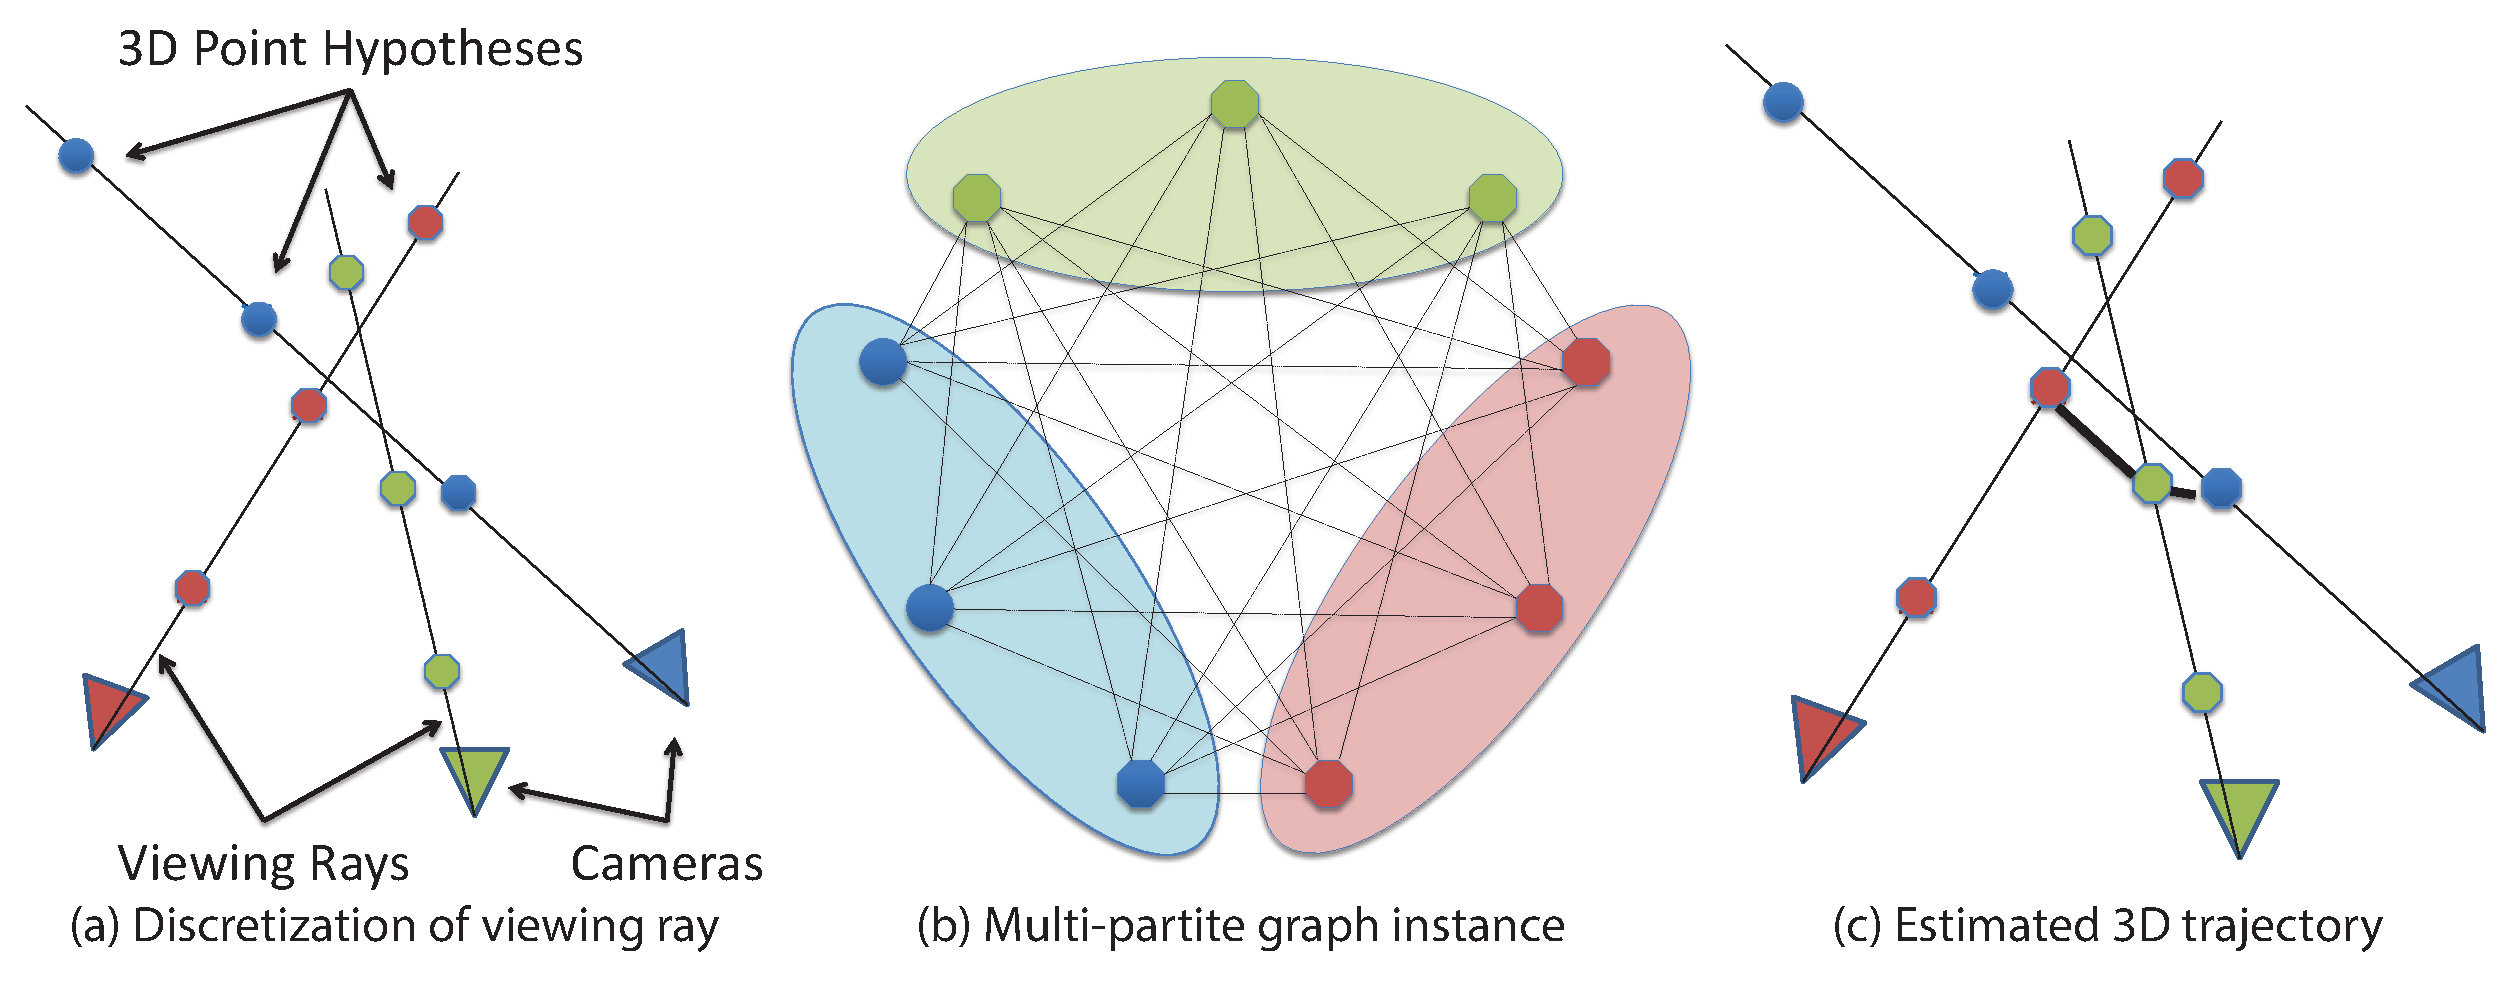
\includegraphics[width=1\columnwidth]{chapter4/resource/gmst_eccv.pdf}
\caption{Illustration of GMST. See the text for more details.}
%\end{subfigure}
\label{fig:gmst}
\end{figure}

\label{sec:gmst}
To determine the \oct, we conceptually have to choose for each ray $\mathbf{X}_i(t_i) $ the 3D point, and simultaneously determine the adjacency $\mathbf{p}$ representing the adjacency relations of the rays $\mathbf{X}_i(t_i) $, which defines the topology of the \oct.
Our discrete-continuous optimization strategy first uses a Generalized Minimum Spanning Tree (GMST) to find adjacency $\mathbf{p}$, and followed by a convex optimization over $\mathbf{t}$ with $\mathbf{p}$ being fixed.

In the discrete optimization step, we map the continuous problem of finding the 3D point along each ray to a discrete problem of selecting a 3D point out of a set of discrete 3D points. Then we determine one 3D point along each ray and the adjacency $\mathbf{p}$ by computing the GMST on an undirected multipartite graph $\cal{G}(V,E)$~\cite{MyungLT_95}. This allows us to simultaneously  determine the topology and the discrete 3D object positions.

An undirected multipartite graph is a graph whose vertices are partitioned into $N$ partite sets $\left\{V_1, \dots, V_N\right\}$ with $\vert V_i \vert = k$, while fulfilling ${\cal V}=V_1 \cup V_2 \cup \dots \cup V_N$ and $V_o \cap V_p = \emptyset, \forall o\neq p$, with $o,p \in \{1, \dots, N \}$. The multipartite graph $\cal{G}(V,E)$ has only edges between the different partite sets  of vertices $V_o$, and all edge cost are non-negative. Now we will detail on how we define the graph $\cal{G}(V,E)$ based on Eq.~\ref{equ:costFunc}.

Each ray $\mathbf{X}_i(t)$ defines a one dimensional constraint on the 3D position of the object. We discretize the ray to obtain a discrete set of potential depth estimates. This leads to a finite set of possible 3D positions along the ray (see Figure \ref{fig:gmst}(a) for an illustration), defining a finite set of 3D point hypotheses %$\mathbf{\hat{X}}_i^o=\mathbf{X}_i (\hat{t}_o)$ with $\vert t_o \vert = k$,
$\{\mathbf{\hat{X}}_i^o|o=1,\dots,k \}$,
where $k$ is the number of the discrete hypotheses along the ray.
In our representation, each 3D point $\mathbf{\hat{X}}_i^o$ establishes node $V_i^o$ in the graph. The set of nodes $\{V_i^o|o=1, \dots, k\}$ related to the ray $\mathbf{X}_i(t)$ of object $i$ defines a partite set of nodes $V_i$ in the graph $\cal{G}(V,E)$. 
Given that no nodes within a group have any connecting edges, it enforces the traversal of the graph to be constrained among partite sets. 
%This is  consistent with the understanding of moving the different instances of an object class in the scene to determine the object class trajectory.

We now define the edge cost of the multipartite graph based on Eq. (\ref{equ:costFunc}).
The multipartite graph only has edges between the nodes from different partite sets.
%Given the properties of the multipartite graph we only insert edges between the nodes that are in different partite sets of nodes.
We define the edge direction $\mathbf{d}_{i,j}$ between any two nodes $V_i^o$ and $V_j^p$ in the partite set $i$ and partite set $j$ respectively, as the consistency of the 3D motion with the motion tangents $\mathbf d_i$ and $\mathbf d_j$ (see Sec. \ref{sec:detection}). This definition comes from the intuition that the edge direction should be compliant with the motion tangent observed in the images. Given the motion of two objects $i$ and $j$ and their respective motion tangents $\mathbf d_i$ and $\mathbf d_j$, it is clear that the motion between the points $\mathbf{X}_i^o$ and $\mathbf{X}_j^p$ (associated with the nodes $V_i^o$ and $V_j^p$) should be close in direction to at least one of the motion tangents $\mathbf d_i$ and $\mathbf d_j$.
%Then one can think that the edge direction $\mathbf{d}_{i,j}$ should be either $\mathbf{d}_i$ or $\mathbf{d}_j$, as is shown in Figure \ref{fig:node_DirectionA}. Any edge parallel to $\mathbf{d}_i$ or $\mathbf{d}_j$ should be encouraged.
Therefore, we define the edge cost $e(V_i^o,V_j^p)$ of the edge between the nodes $V_i^o$ and $V_j^p$ as

\begin{equation}
\label{eq:edgecost}
e(V_i^o,V_j^p)=\text{min}(\|\mathbf{d}_i\times(\mathbf{X}_i^{o}-\mathbf{X}_j^{p})\|_2^2, \|\mathbf{d}_j\times(\mathbf{X}_i^{o}-\mathbf{X}_j^{p})\|_2^2) +\lambda\|\mathbf{X}_i^{o}-\mathbf{X}_j^{p}\|_2^2.
\end{equation}
If only considering the first term in Eq. (\ref{eq:edgecost}), edges with 3D motion directions that are approximately parallel to $\mathbf{d}_i$ or $\mathbf{d}_j$ have lower  cost than those are at an angle to both $\mathbf{d}_i$ and $\mathbf{d}_j$. For instance, %for the edge cost from Eq. (\ref{eq:edgecost}),
Edge 1 and Edge 3 in Figure \ref{fig:node_DirectionB} have a relatively lower cost than Edge 2 because Edge 1 is parallel to $\mathbf{d}_j$ and Edge 3 is parallel to $\mathbf{d}_i$.

\subsection{GMST}
\begin{figure}[t]
\centering
\subfloat[]{
    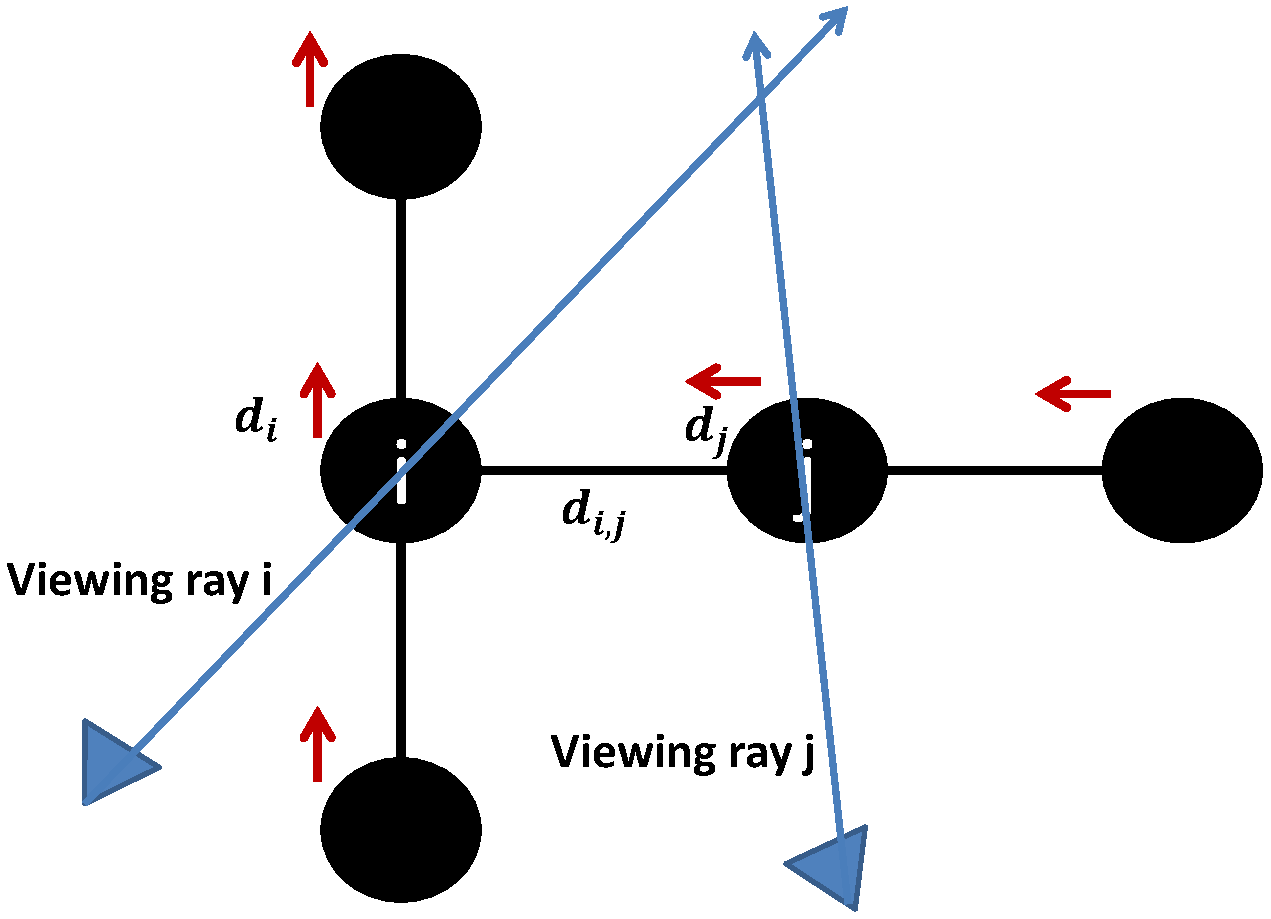
\includegraphics[height=0.19\textheight]{chapter4/resource/nodeDirection1_cropped.pdf}
    \label{fig:node_DirectionA}
}
\subfloat[]{
    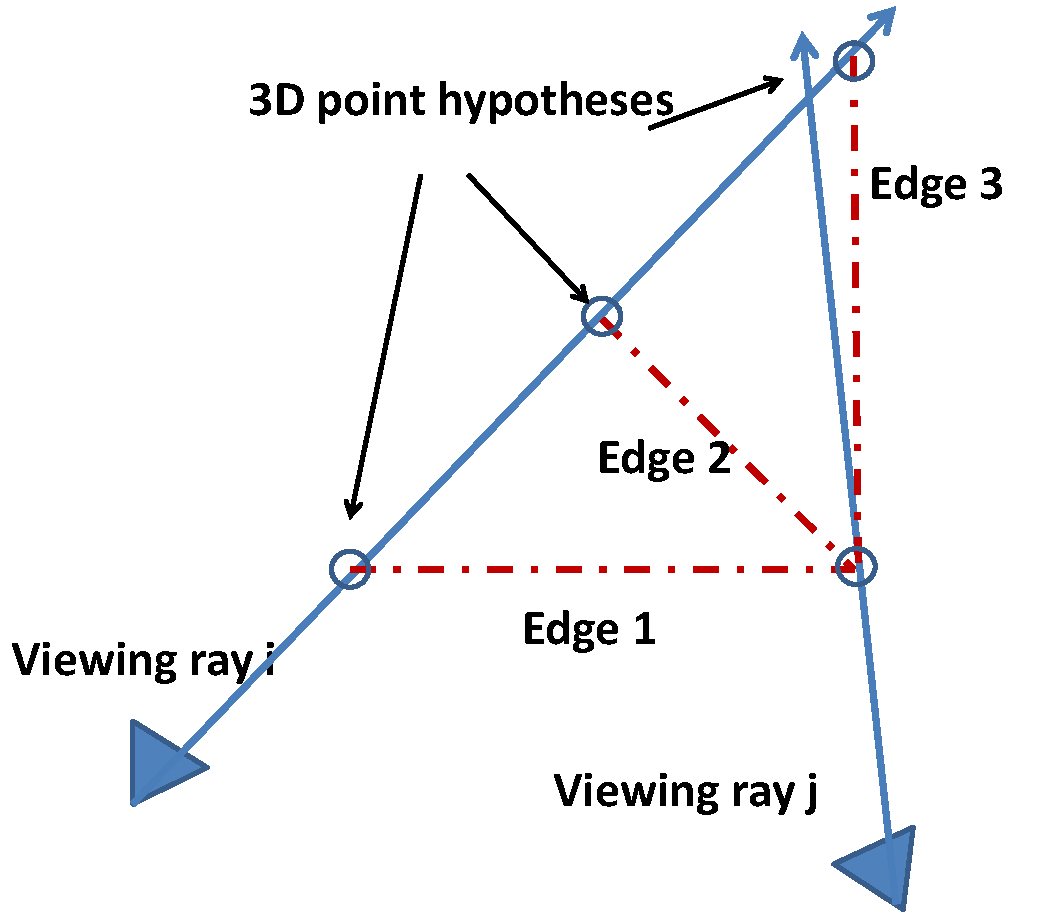
\includegraphics[height=0.19\textheight]{chapter4/resource/nodeDirection2_cropped.pdf}
    \label{fig:node_DirectionB}
}
\subfloat[]{
    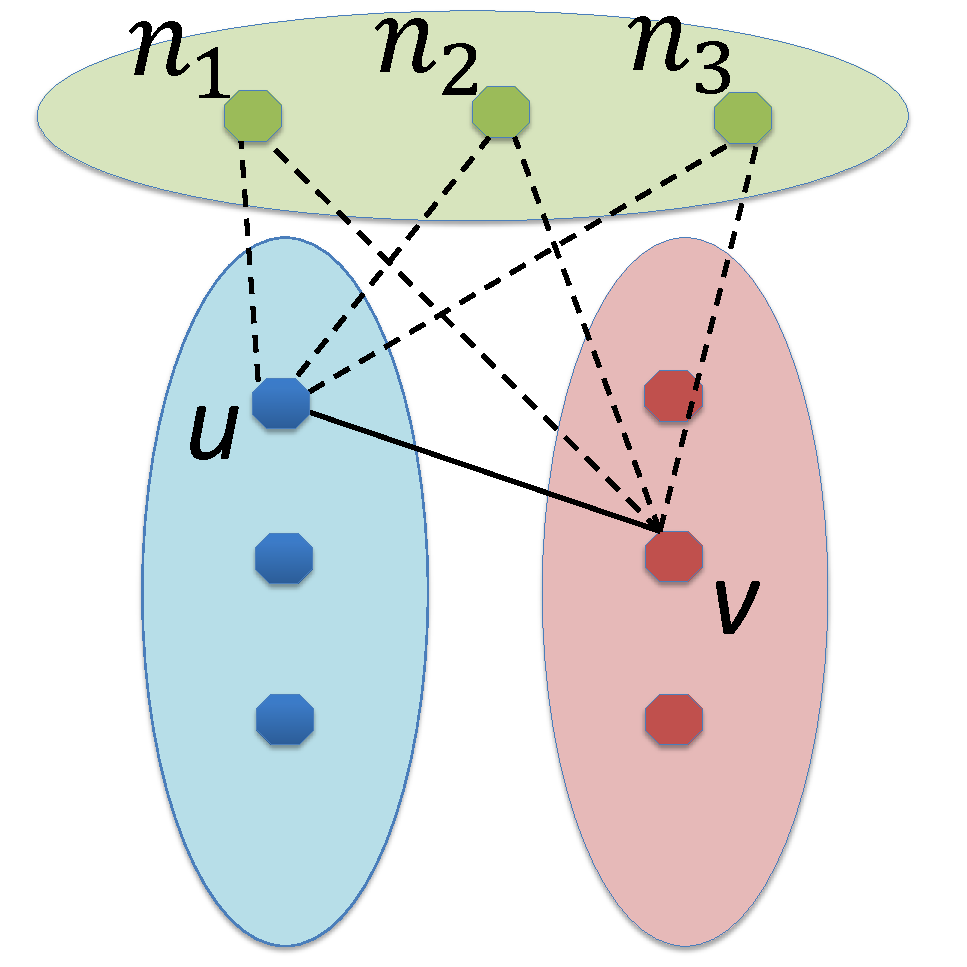
\includegraphics[height=0.19\textheight]{chapter4/resource/edgeReduction_cropped.pdf}
    \label{fig:node_edgeRemove}
}

\caption{In Figure \ref{fig:node_DirectionA}, the black nodes shows the real positions of dynamic objects. The red vector represents the direction associated with each object. In the shown example, $\mathbf{d}_{i,j}$ equals $\mathbf{d}_{i}$.  }
%\end{subfigure}
\label{fig:nodeDirection}
\end{figure}

A Generalized Minimum Spanning Tree (GMST) on the graph $\cal{G}(V,E)$ is a tree of minimal cost that spans \emph{exactly one node} from each partite set $V_i$. GMST problem degenerates to a typical minimum spanning tree problem \cite{Cormen:2001:IA:580470} if each of the partite sets contains only one node.
For our proposed graph, it means a GMST includes exactly one 3D point from each ray. Furthermore, GMST prefers the edge $e(V_i^o,V_j^p)$ that has small value of $\|\mathbf{X}_i^o-\mathbf{X}_j^p\|^2$ and is compliant with the motion tangents in the images, as those edges have lower edge cost. Accordingly, a GMST is our desired solution for estimating the \oct. Notice that if we sample infinite number of 3d points along each viewing ray, the corresponding GMST problem is equivalent to the original cost function Eq. (\ref{equ:costFunc}).% before discretization for the multipartite graph formulation.

The multipartite graph defined above contains a large amount of edges, which increases the complexity of computing the GMST.
We use a deterministic way introduced by Ferreira et al. \cite{Ferreira_ESWA2012} to remove those edges that are guaranteed not to be included in the GMST. Here we use a specific toy example in Figure \ref{fig:node_edgeRemove} to illustrate the method. If the cost of edge $(u,v)$ is larger than any cost of the 6 edges $(u,n_l)$ and $(v,n_l)$, $l=1,2,3$, the edge $(u,v)$ is safe to be removed. A simple proof is that if edge $(u,v)$ exists in the computed GMST, we could remove edge $(u,v)$ and replace it by one of the 6 edges to obtain a new GMST with lower cost. Therefore, edge $(u,v)$ can not be present in the GMST. Moreover, it is plausible to explore other ways to remove edges based on given prior information. For instance, if it is known the pairwise neighboring 3D objects are close in 3D space, we can safely remove the edges that connects two farther point hypotheses by applying a threshold.

The GMST problem was first introduced by Myung \citet{MyungLT_95} and was extensively studied in the past two decades \cite{Feremans_LL02,MyungLT_95,Oncan_CL08,Ferreira_ESWA2012,Dror_EJOR} due to its wide applications in  telecommunications, agriculture watering, and facility distribution design \cite{MyungLT_95,Dror_EJOR}. Unlike the minimum spanning tree (MST) problem, which can be solved in polynomial time, finding the GMST is proved to be NP-hard \cite{MyungLT_95}. Myung \etal \cite{MyungLT_95} and Feremans \etal \cite{Feremans_LL02} propose several integer programming formulations for the GMST problem. However, those provide no guarantee of efficiency, especially when the problem scale is large. The computational challenge of the GMST problem has led to the development of metaheuristics \cite{Oncan_CL08,Ferreira_ESWA2012} that search the hypothesis space, and are empirically shown to be effective.

We exploit the state-of-the-art GRASP-based approach proposed by Ferreira \etal \cite{Ferreira_ESWA2012}. GRASP (Greedy Randomized Adaptive Search Procedure) is a metaheuristic that consists of iterations made up two phases: 1) solution construction and 2) solution improvement through local search. \citet{Ferreira_ESWA2012} proposed the method considering several solution construction algorithms, a local search procedure, and two additional mechanisms: path-relinking and iterative local search. We refer readers to their paper \cite{Ferreira_ESWA2012} for more details.

The output of GMST computation is the estimation of the 3D points $\mathbf{\widehat{X}}$ and the adjacency topology of the \oct. Then $\mathbf{d}_{i,j}$ equals one of $\mathbf{d}_i$ and $\mathbf{d}_j$  that has smaller angle to the vector $\mathbf{\widehat{X}}_i - \mathbf{\widehat{X}}_j$,
\begin{equation}
\mathbf{d}_{i,j}= \underset{\mathbf{d}\in{\{\mathbf{d}_i, \mathbf{d}_j}\} }{\arg\!\max}(|\mathbf{d} \cdot (\mathbf{\widehat{X}}_i - \mathbf{\widehat{X}}_j)| ).
%\mathbf{d_{i,j}} = \text
\end{equation}
%The solution described by the GMST provides us with the discretized 3D points $\mathbf{X}_i^{o}$ as the nodes of the GMST and with the adjacency $\mathbf{p}$ of nodes as defined by the GMST. This represents the rays of the objects as a discrete \oct. While the adjacency is naturally a discrete entity the 3D points of the object along the motion path are naturally continuous entities. Hence, we accept
We fix the adjacency $\mathbf{p}$ given by the GMST, and add a final continuous refinement step for the 3D object position $\mathbf{\hat{X}}_i$, through a convex program optimization over variable $\mathbf{t}$
%To achieve this we fix the adjacency $p$ and only optimize over the object positions $\mathbf{t}$ in Equation (\ref{equ:costFunc}). This leads to the following optimization problem:
\begin{equation}
\underset{\mathbf{t}} { \text{min} }
\sum_{(i,j)\in{\mathbf{p}}}{\|\mathbf{d}_{i,j}\times(\mathbf{X}_i-\mathbf{X}_j)\|_2^2 + \lambda\|\mathbf{X}_i-\mathbf{X}_j\|_2^2}
\label{equ:costFunc_continuous}
\end{equation}
%Solving the convex program in Equation (\ref{equ:costFunc_continuous}) provides the continuous solution for the 3D object positions along the \oct.


\subsection{Reconstructability Analysis} \label{sec:analysis}

Now we analyze the reconstructability of the proposed method, i. e. determining under which conditions the solution of Eq. (\ref{equ:costFunc}) generates accurate 3D points. The direct analysis of Eq (\ref{equ:costFunc}) is difficult, as it needs to determine in which situation the adjacency $\mathbf{p}$ with minimum cost, out of $N^{N-2}$ possible adjacencies (\cite{wiki_cayley_alg}), corresponds to the \oct. %This requires us to relates the camera centers and real 3D object positions.
We find that having the motion tangent constraint reduces the possibility of finding the wrong adjacency $\mathbf{p}$. Hence, we focus on  the reconstructability of the continuous method Eq. (\ref{equ:costFunc_continuous}) given the adjacency $\mathbf{p}$.

Assume we already know the ground truth 3D point $\mathbf{{X}}_i^*$ of object $i$, $i=1,\dots,N$. Given that $\mathbf{{X}}_i^*$ is present on the viewing ray $\mathbf{X}_i$, we move the camera center $\mathbf{C}_i$ to $\mathbf{X}_i^*$ along the ray $\mathbf{X}_i(t)$ in direction $\mathbf{r}_i$. Then any point on the line that passes through $\mathbf{X}_i^*$ and has ray direction $\mathbf{r}_i$ can be represented as $\mathbf{X}_i (s_i)= \mathbf{X}_i^* + s_i \cdot \mathbf{r}_i$, where $s_i$ is the signed distance (not the positive distance as defined by the $t_i$). Then Eq. (\ref{equ:costFunc_continuous}) can be reformulated as:
\begin{equation}
\label{equ:costFunc_analysis}
\underset{\mathbf{s}} { \text{min} }
\sum_{(i,j)\in{\mathbf{p}}}{\|\mathbf{d}_{i,j}\times(\mathbf{X}_i(s_i)-\mathbf{X}_j(s_j))\|_2^2 + \lambda\|\mathbf{X}_i(s_i)-\mathbf{X}_j(s_j)\|_2^2}, \\
\end{equation}
where $\mathbf{s}=[s_1, \dots, s_N]$. Though $s_i$ is signed distance and $t_i$ is positive distance, minimizing Eq. (\ref{equ:costFunc_continuous}) and Eq. (\ref{equ:costFunc_analysis}) still output the same 3D point positions, as long as the computed 3D points in Eq. (\ref{equ:costFunc_analysis}) are in front of the camera centers. We will see that this is normally true, because the computed 3D points are typically close to their ground truth position if the system is well-conditioned.

We denote the solution of Eq. (\ref{equ:costFunc_analysis}) as $\mathbf{s}^\text{opt}$. The true 3D points are ideally reconstructed if $\mathbf{s}^\text{opt}=0$, since $\mathbf{X}_i(0)$ equals to $\mathbf{{X}}_i^*$ given $\mathbf{s}^\text{opt}=0$.
More specifically, $\mathbf{s}^\text{opt}$ equals the signed Euclidean distance between the 3D points produced by Eq. (\ref{equ:costFunc_continuous}) and the ground truth $X_i^*$.
Therefore, $\|\mathbf{s}^\text{opt}\|$ is the error of the estimated 3D points by Eq. \ref{equ:costFunc_continuous}.
In the remaining of this section, we further analyze when $\|\mathbf{s}^\text{opt}\|$ is small to understand the quality of the estimated 3D points. %achieved approximation.

The minimum value of Eq. (\ref{equ:costFunc_analysis}) is achieved at the point where the first derivative relative to $\mathbf{s}$ equals 0. This produces a linear equation system $\mathbf{A}\mathbf{s}^\text{opt}= \mathbf{b}$, where the $i$th row and $j$th column of matrix $\mathbf{A}$ is
\begin{equation}
A_{ij}= \begin{cases}
%\mathbf{r}_i\cdot\mathbf{r}_j, & \text{if } (i,j)\in T \text{ and } i\neq j \\
\lbrack(\mathbf{r}_i\cdot\mathbf{d}_{i,j})\mathbf{d}_{i,j}-(1+\lambda)\mathbf{r}_i\rbrack\cdot\mathbf{r}_j  & \text{if } i\neq j \text{ and } (i,j)\in \mathbf{p}\\
0, & \text{if } i\neq j \text{ and } (i,j)\notin \mathbf{p}\\
\sum_{(i,k)\in{\mathbf{p}}}{\lbrack 1+\lambda - (\mathbf{r}_i\cdot\mathbf{d}_{i,k})^2 \rbrack } & \text{if } i=j
\end{cases}
\label{equ:A}
\end{equation}
The $i$th element of vector $\mathbf{b}$ is
\begin{equation}
b_i=\sum\nolimits_{(i,k)\in{\mathbf{p}}}(\mathbf{X}_k^*-\mathbf{X}_i^*)\cdot \lbrack(1+\lambda)\mathbf{r}_i - (\mathbf{r}_i\cdot \mathbf{d}_{i,k})\mathbf{d}_{i,k} \rbrack
\label{equ:b}
\end{equation}
Eq. (\ref{equ:A}) and Eq. (\ref{equ:b}) have the following interesting properties:
\begin{enumerate}
\item If $\mathbf{b}$ is 0, $\mathbf{s}^\text{opt}$ equals 0, which means the solution of Eq. (\ref{equ:costFunc_continuous}) recovers the true 3D points. There are a few situations  $\mathbf{b}$ equal 0. (1) In the case of a static object $\mathbf{X}_i^* = \mathbf{X}_k^*$, $\mathbf{b}$ equals 0 based on Eq. (\ref{equ:b}). (2) Careful observation reveals that if $\lambda$ is set to $0$, in Eq. (\ref{equ:b}) the vector $(1+\lambda)\mathbf{r}_i - (\mathbf{d}_{i,k}\cdot \mathbf{r}_i)\mathbf{d}_{i,k}$ is perpendicular to vector $\mathbf{X}_i^*-\mathbf{X}_k^*$ (Figure \ref{fig:b_lambda0}), hence $b_i=0$. However, we will show that with $\lambda=0$, the linear system $\mathbf{A}\mathbf{s}= \mathbf{b}$ is unstable due to the high condition number of $\mathbf{A}$. (3) As shown in Figure \ref{fig:b_lambdaBiggerthan0}, as $\lambda$ increases from 0, the two vectors slowly deviate from being perpendicular. Therefore, $b_i$ is likely to be small if $\lambda$ is close to 0.
\item Since we can not control 3D positions and there are typically small measurement errors in $\mathbf{d}_{ij}$, $\mathbf{b}$ does not exactly equal to 0. This can be regarded as a small disturbance of $\mathbf{b}$ around $\mathbf{0}$. For the linear system $\mathbf{A}\mathbf{s}^\text{opt}= \mathbf{b}$, one can think of the condition number $\kappa(\mathbf A)$ as being (roughly) the rate at which the solution, $\mathbf{s}^{\text{opt}}$, will change with respect to a change in $\mathbf{b}$. $\kappa(\mathbf A)$ is available as it solely depends on $\mathbf{r}_i$, $\mathbf{d}_{i,j}$ and $\lambda$, but not on the ground truth 3D points $\mathbf{X}^*$. Therefore, we can roughly estimate the reliability of the reconstructed 3D points by computing $\kappa(\mathbf A)$. Moreover, we empirically found that the condition number of matrix $\mathbf{A}$ is inversely related to $\lambda$. The condition number shown in Figure \ref{fig:conditionNum_lamda} is computed using 100 random cameras, and averaged over 200 trials. We can see $\kappa(\mathbf A)$ is large if $\lambda$ is close to 0 and drop dramatically with small $\lambda$. Then $\kappa(\mathbf A)$ decreases monotonically and slowly as $\lambda$ increases. In our experiments, we choose $\lambda=\frac{1}{15}$ as a balance of having good chance of small $\mathbf{b}$ and the stability of the linear system.
\end{enumerate}
In conclusion, if the adjacency $\mathbf{p}$ is correctly found, the reconstructabililty of the object class trajectory mainly depends on the condition number of the linear system. Given the well-conditioned system and correct motion tangent $\mathbf{d}_{i,j}$, we are able to reconstruct the 3D positions close to the ground truth.

\begin{figure}[t]
\centering
%\begin{subfigure}[b]{0.3\textwidth}
\subfloat[$\lambda=0$]{
    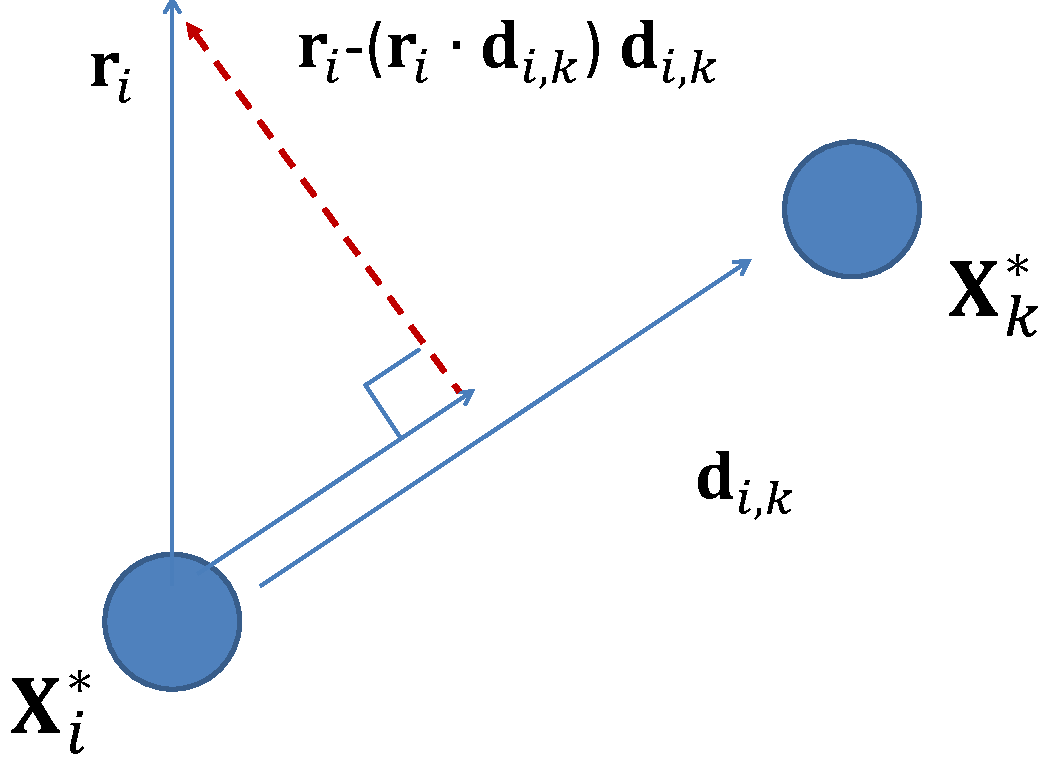
\includegraphics[height=0.17\textheight]{chapter4/resource/analysis_1_cropped.pdf}
    \label{fig:b_lambda0}
}
\subfloat[$\lambda>0$]{
    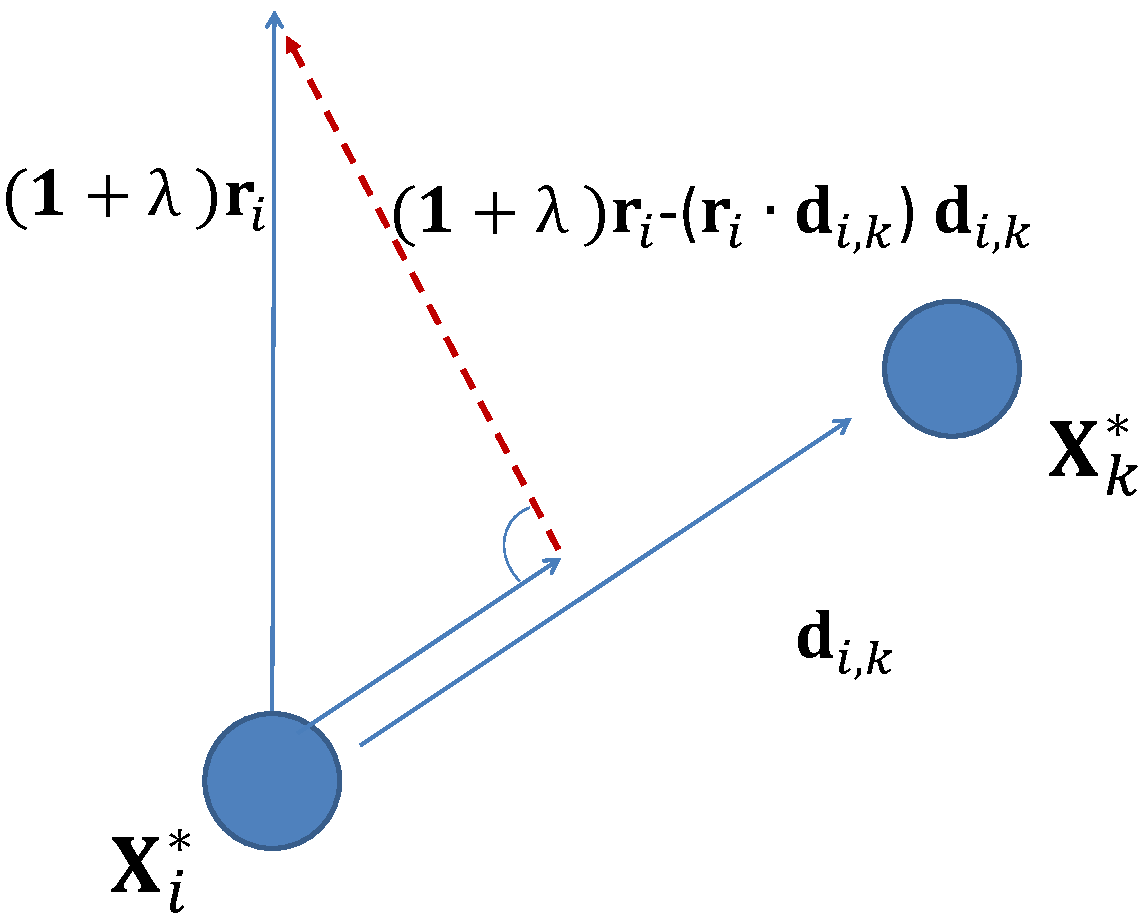
\includegraphics[height=0.17\textheight]{chapter4/resource/analysis_2_cropped.pdf}
    \label{fig:b_lambdaBiggerthan0}
}
\subfloat[$\kappa(\mathbf{A})$ versus $\lambda$]{
    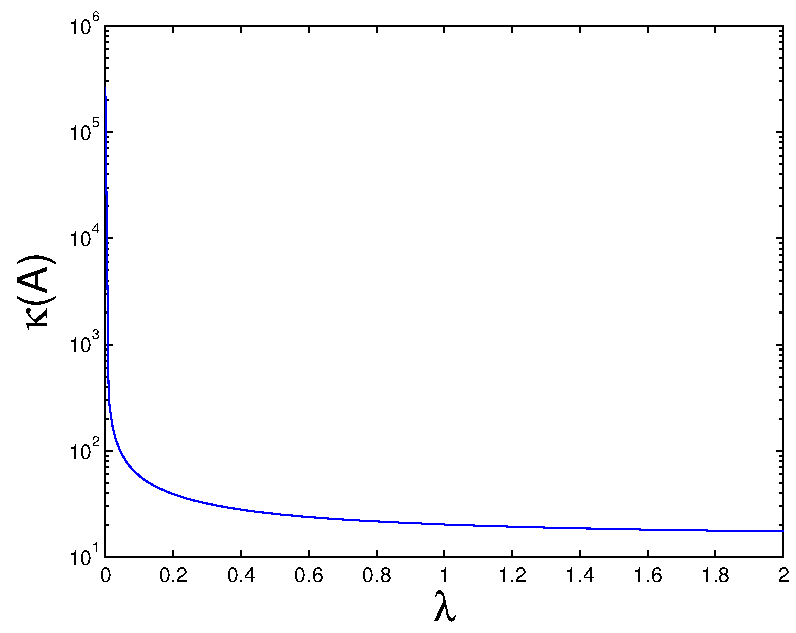
\includegraphics[height=0.17\textheight]{chapter4/resource/conditionNum_lamda.pdf}
    \label{fig:conditionNum_lamda}
}
\caption{Left two: Plot of Eq. (\ref{equ:b}) with $\lambda=0$ and $\lambda>0$. Right: $\kappa(\mathbf{A})$ given different $\lambda$.}
\label{fig:b}
\end{figure}

%%%%%%%%%%%%%%%%%%%%%%%%%%%%%%%%%%%%%%%%%%%%%%%%%%%%%%%%%%%%%%%%%%%%%%%%%%%%%%%%%%%%%%%%%%%%%%%%%%%

%%%%%%%%%%%%%%%%%%%%%%%%%%%%%%%%%%%%%%%%%%%%%%%%%%%%%%%%%%%%%%%%%%%%%%%%%%%%%%%%%%%%%%%%%%%%%%%%%%%
\section{Object Detector and Motion Tangent Estimation}
\label{sec:face_detection}
Before presenting our experimental evaluation, we first briefly describe the particular object detectors we use in our experiments.
Single image based object detection is a well studied problem in computer vision with a wide variety of method readily available~\cite{Zhang2006Local,Dalal2005HOG,lsvm-pami}. Similarly, there is a large number of motion tangent estimation methods in the literature~\cite{Blanz2003face,Gu20063D,jain2010fddb,jones2003fast}.
%While a combination of those methods would yield the desired detections and motion tangents,
We opt for leveraging the method that jointly determines the face position and its motion tangent direction~\cite{Xiangxin_CVPR12}.
%We applied the unified method proposed by Xiangxin \etal \cite{Xiangxin_CVPR12} to jointly detect pedestrian faces and estimate their corresponding motion tangents.
%The method  models the faces as mixtures of tree structures based on shared facial landmarks. 
In our experiments,
%a single template is shared for all 99 facial landmark parts across all 13 mixtures.
the detection threshold is set to $-0.35$ to avoid false detections, as the false alarm may disturb our algorithm. Our chosen detectors provide a motion tangent of object $i$ that is  quantized every $\theta=15^{\circ}$ in the range of $-90^{\circ}$ and $90^{\circ}$.

%To further improve the detection of pedestrians at larger distances we default to a deformable parts
For cars and pedestrians with small faces in the image, we default to the deformable parts
detector~\cite{lsvm-pami,voc-release5}. %, which could also be used for the detection of cars. %This detector utilizes HOG features.
We used the pre-trained model with detection threshold $0.35$.
%The deformable part-based models are discriminatively learned using latent SVMs.
%We used the pre-trained pedestrian model from the INRIA person dataset~\cite{Dalal2005HOG} with detection threshold $0.35$.
% and the \en{ do we have a car experiment? If not we need to take the car out here} car model from the PASCAL dataset~\cite{pascal-voc-2010} with detection threshold $0.1$.
%We again chose higher detection thresholds to avoid false positives. Next we will describe the experimental evaluation of our \jost.
The moving directions of the pedestrians and cars are estimated using the 3D point cloud (output of VisualSFM) of the background wall by assuming the dynamic objects move parallel to the wall. This is normally true for the Manhattan Scene. Some of the detection results are shown in Figure \ref{fig:detection}.
%\begin{figure}[t]
%\centering
%\subfigure[Face detection]{
%\subfigure{
%    \includegraphics[width=0.4\textwidth]{resource/detection/face_detection.png}
%    \label{fig:face_detection}
%    }
%\quad
%\subfigure[Pedestrian detection]{
%\subfigure{
%    \includegraphics[width=0.4\textwidth]{resource/detection/ped_detection.png}
%    \label{fig:pedestrian_detection}
%    }
%\caption{Detected objects and estimated motion tangents using different detectors.}
%\label{fig:detection}
%\end{figure}

\begin{figure}[t]
\centering
\begin{tabular}{c c c}
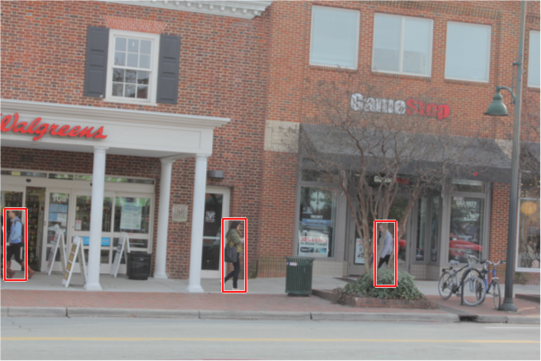
\includegraphics[width=0.3\textwidth]{chapter4/resource/ped_seq_3.png} & 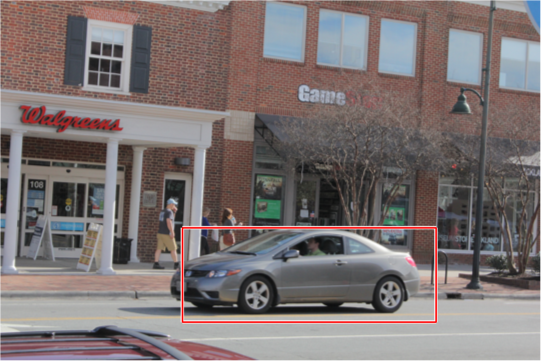
\includegraphics[width=0.3\textwidth]{chapter4/resource/IMG_3375.png} &
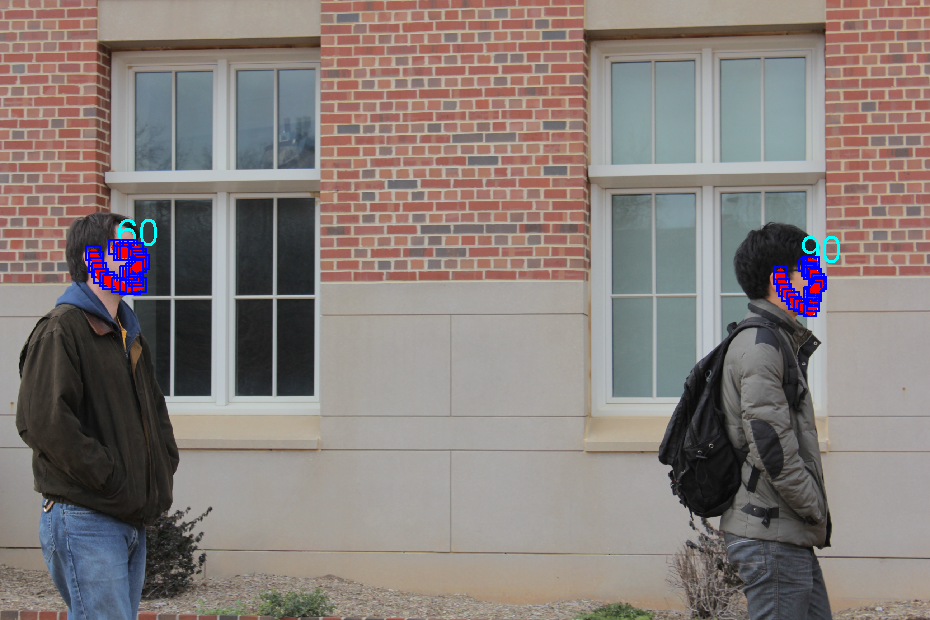
\includegraphics[width=0.3\textwidth]{chapter4/resource/IMG_3000-alldect.png}  \\
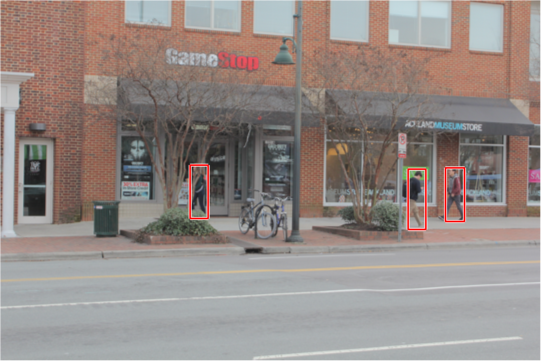
\includegraphics[width=0.3\textwidth]{chapter4/resource/ped_seq_4.png} &
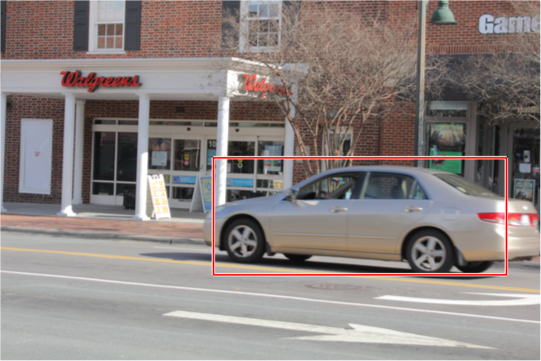
\includegraphics[width=0.3\textwidth]{chapter4/resource/IMG_3365.png} &
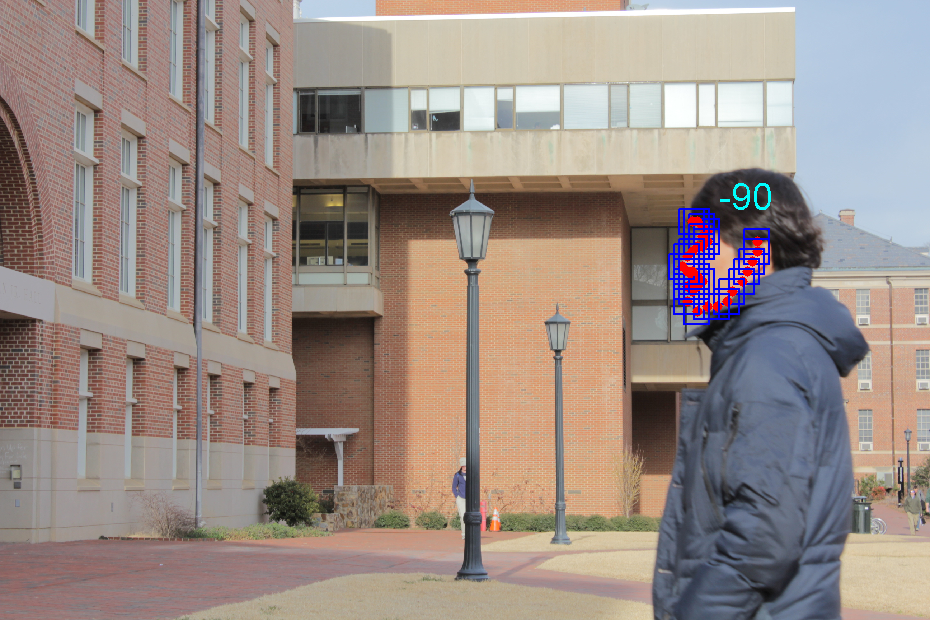
\includegraphics[width=0.3\textwidth]{chapter4/resource/IMG_3073-alldect.png}
\end{tabular}
\caption{Detected objects and estimated motion tangents using different detectors.}
\label{fig:detection}
\end{figure}


%%%%%%%%%%%%%%%%%%%%%%%%%%%%%%%%%%%%%%%%%%%%%%%%%%%%%%%%%%%%%%%%%%%%%%%%%%%%%%%%%%%%%%%%%%%%%

%%%%%%%%%%%%%%%%%%%%%%%%%%%%%%%%%%%%%%%%%%%%%%%%%%%%%%%%%%%%%%%%%%%%%%%%%%%%%%%%%%%%%%%%%%%%%
\section{Experiments}
We evaluate our algorithm on both synthetic and real datasets.
The GMST algorithm used in our method \cite{Ferreira_ESWA2012} searches the hypothesis space, which stops either the GMST cost is under a preset value or the run time reaches a preset limit. For all experiments, we use the time limit to stop searching, given the lack of an adequate {\em a priori} approximation of the true  GMST cost for each dataset.
\begin{table} [b]
\centering
\begin{tabular}{|c|c|c|c|c|c|c|}  \hline
               & single line & T junction & double lines & half circle & sine wave & cross \\
  \hline
  $\text{error}_A$ & 0.5963 & 1.9688 & 1.5169 & 2.3751  & 2.3705 & 3.4111\\
  \hline
  $\text{error}^*_A$ & 0.4263 & 1.9148 & 1.4982 & 2.3340  & 2.3516 & 3.4030 \\
  \hline
  $\text{error}_B$ & 0.2151 & 0.2126 & 0.7824 & 0.2281& 0.2578 &0.2251 \\
  \hline
  $\text{error}^*_B$ & 0.0287 & 0.0944 & 0.7692 & 0.1074 & 0.2305 & 0.1308\\
  \hline
\end{tabular}
\caption{ The table shows the average errors. The subscript represents camera setup. The absence of asterisk represents the GMST algorithm output, and the asterisk is the refined output of Eq. (\ref{equ:costFunc_continuous}). Notice that in ground truth 3D points, the average distance between every pair of nearest points  equals 1. }
\label{fig:syntheticDataResult}
\end{table}
%To access performance of our \jost~,we evaluate its performance on both synthetic and real data.


\begin{figure}[t]
\centering
    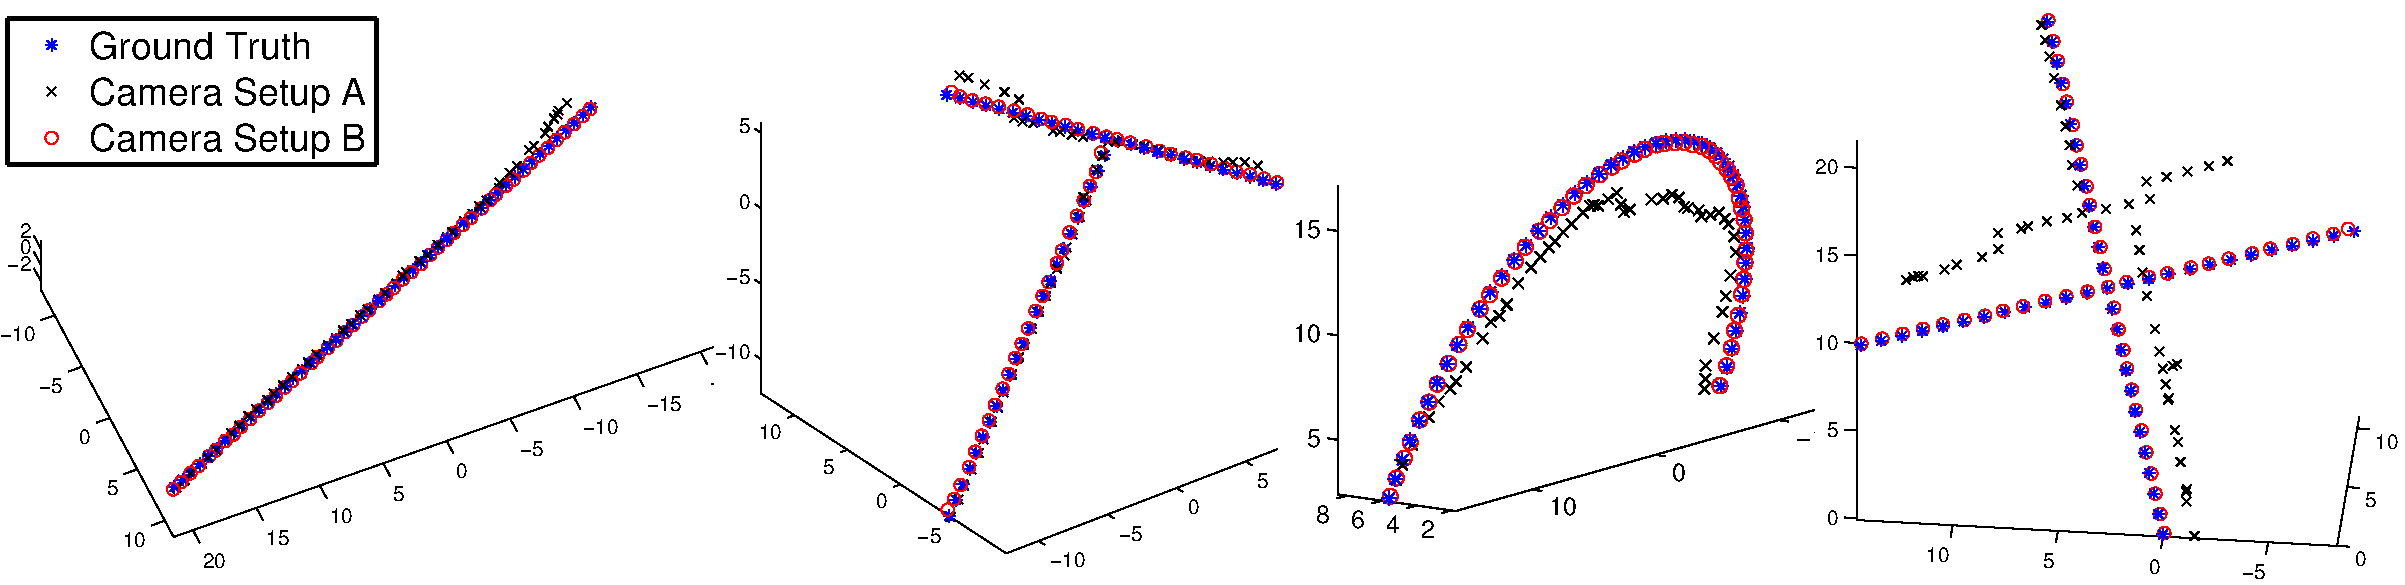
\includegraphics[width=0.98\textwidth]{chapter4/resource/allfig.pdf}
\caption{Example results for line path, T-junction path, half circle and crossed paths.}
\label{fig:synthetic}
\end{figure}


\begin{figure}[t]
\centering
\subfloat{
    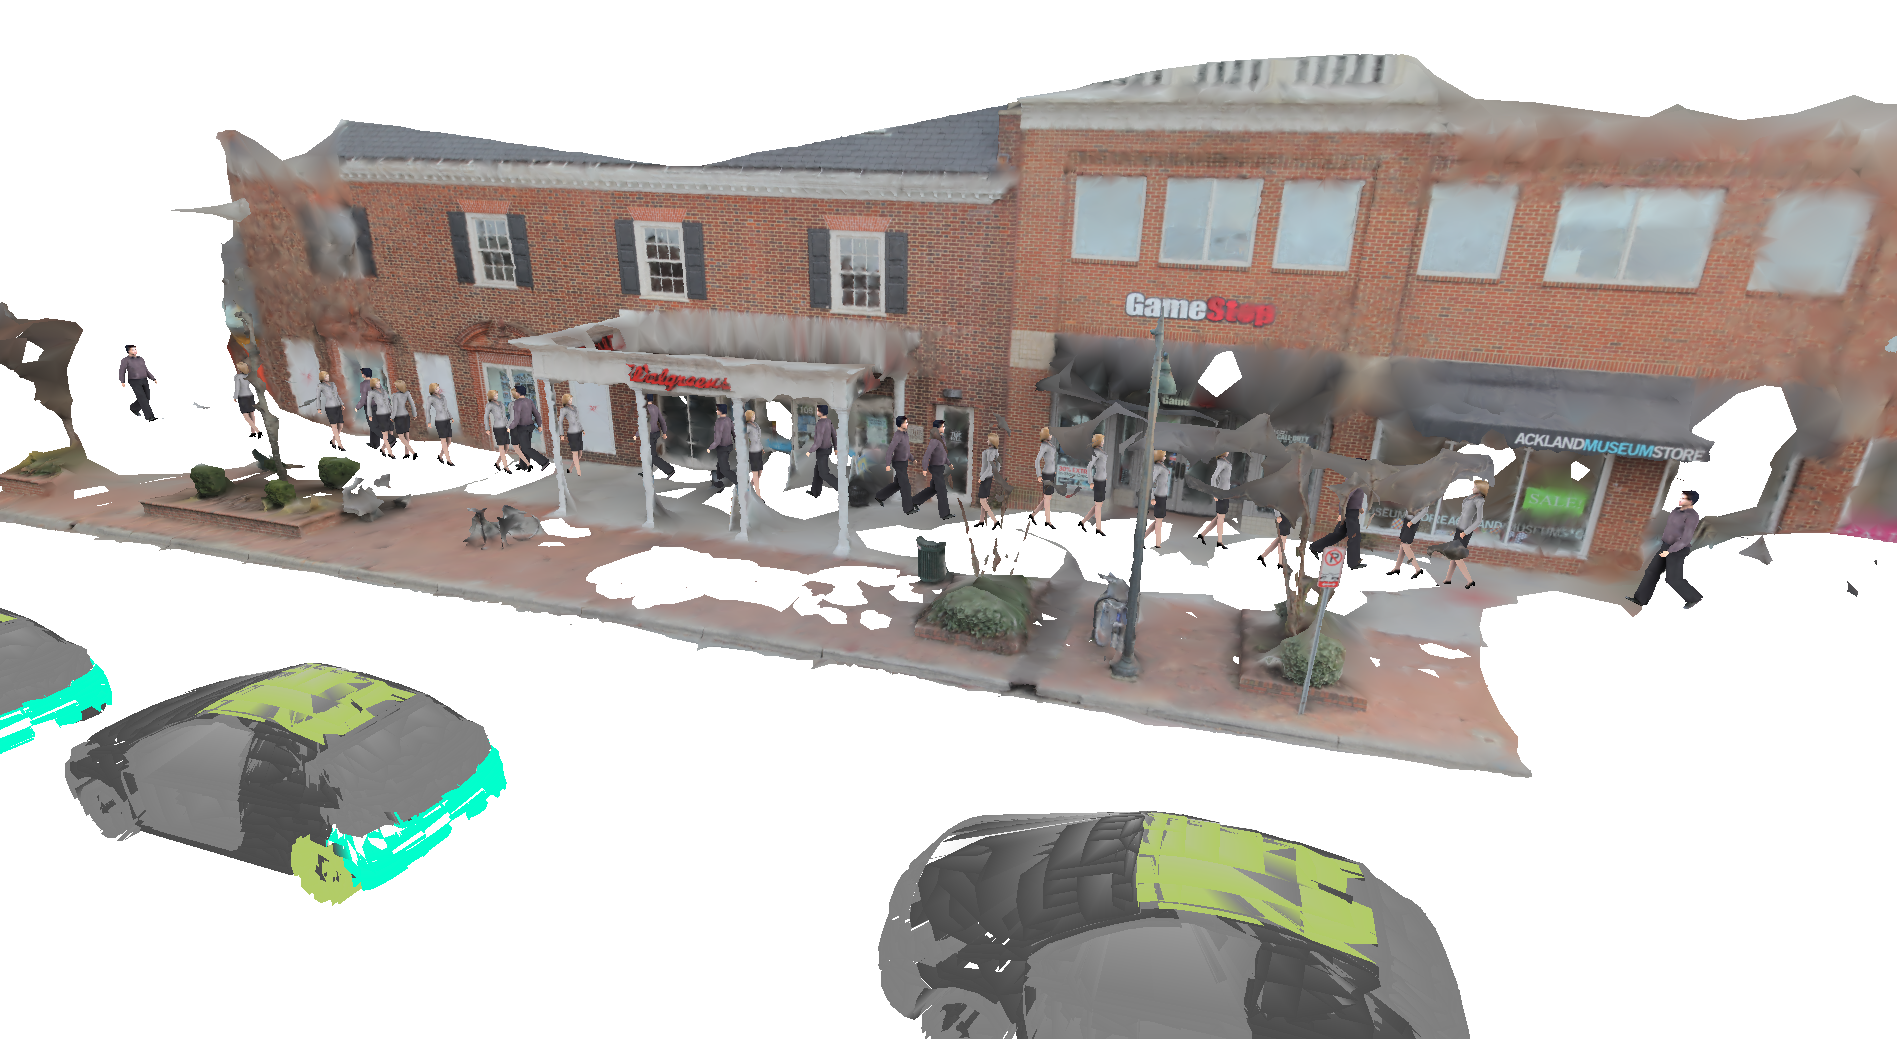
\includegraphics[height=0.15\textheight]{chapter4/resource/snapshot03.png}
    }
\subfloat{
    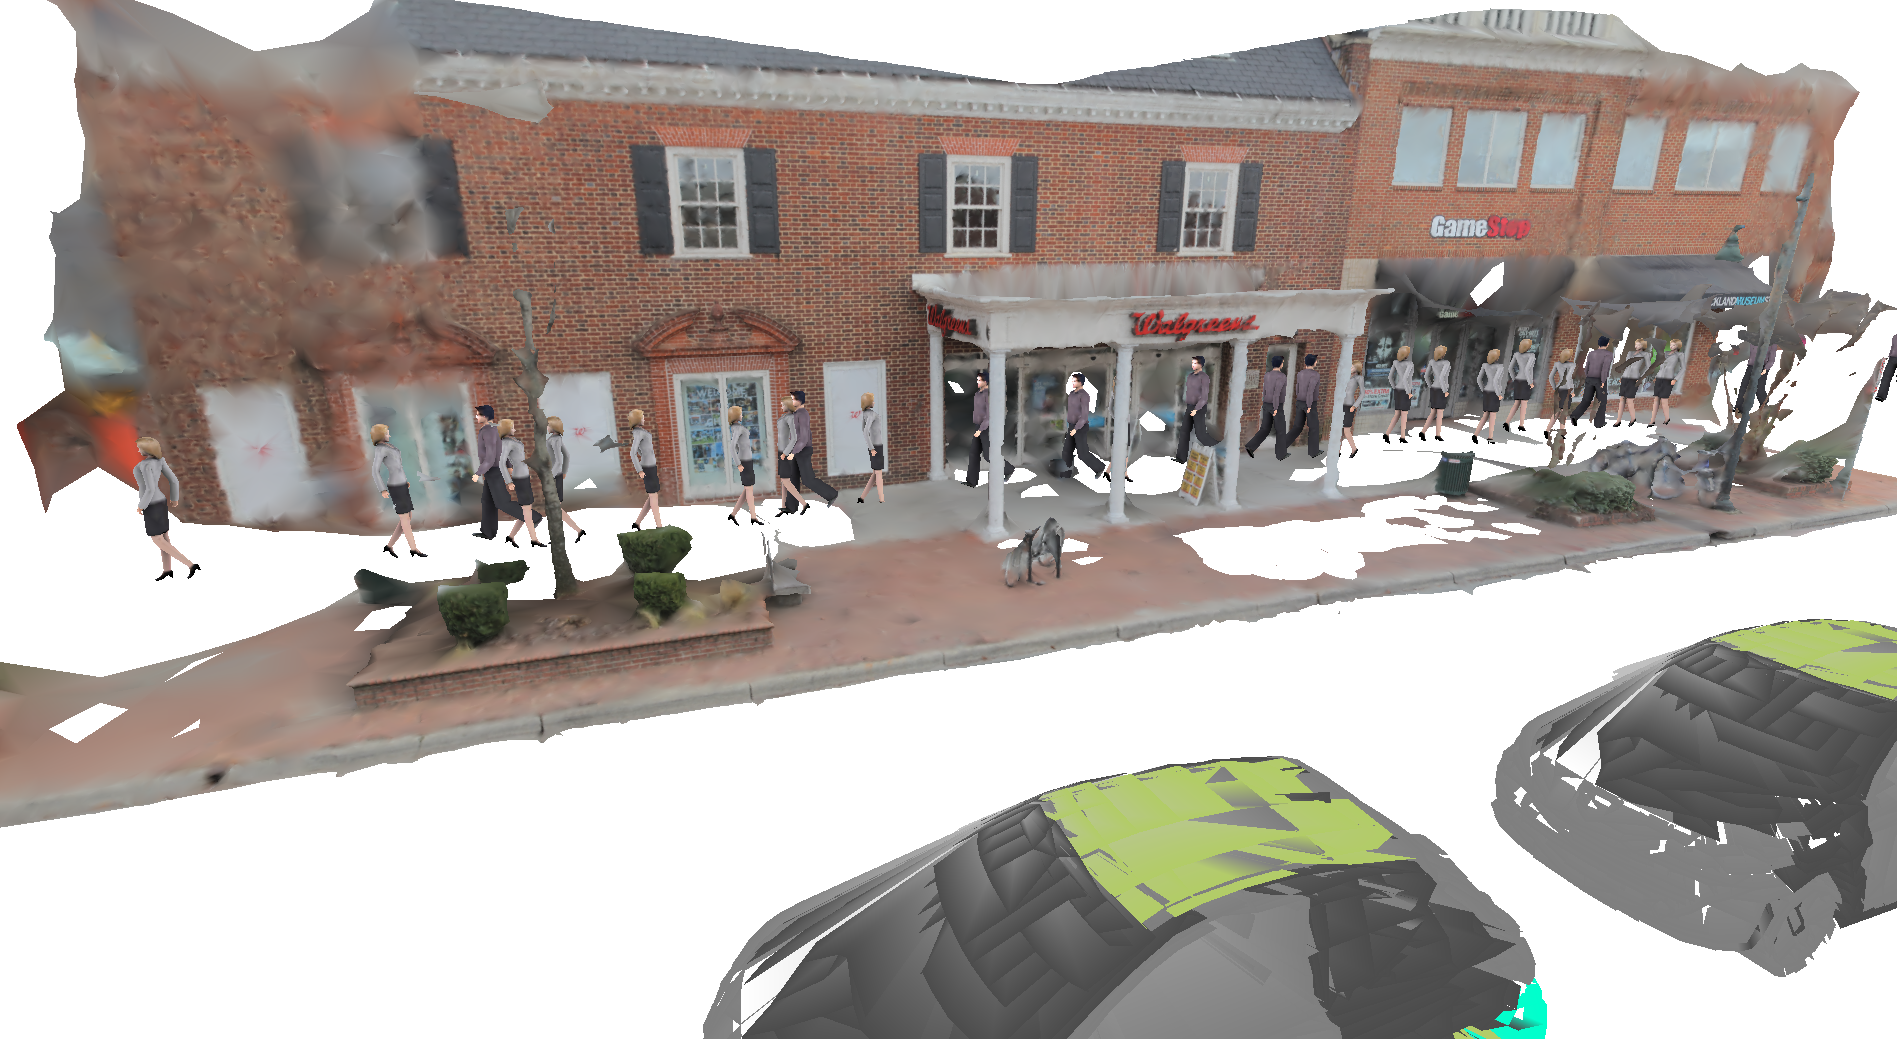
\includegraphics[height=0.15\textheight]{chapter4/resource/snapshot05.png}
    }\\
\subfloat{
    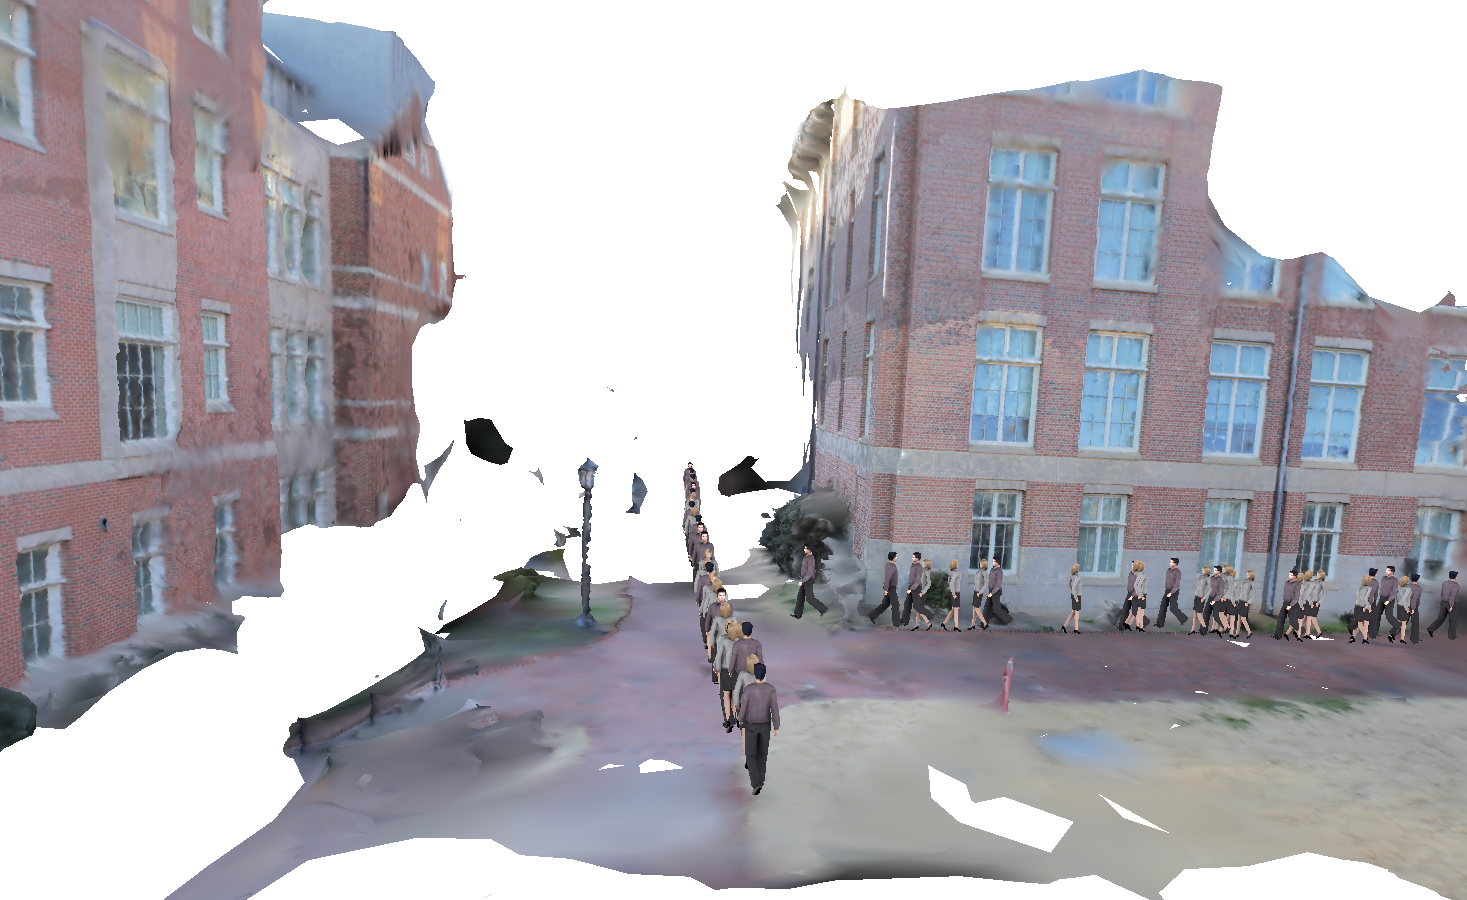
\includegraphics[height=0.18\textheight]{chapter4/resource/tjunction1.PNG}
}
\subfloat{
    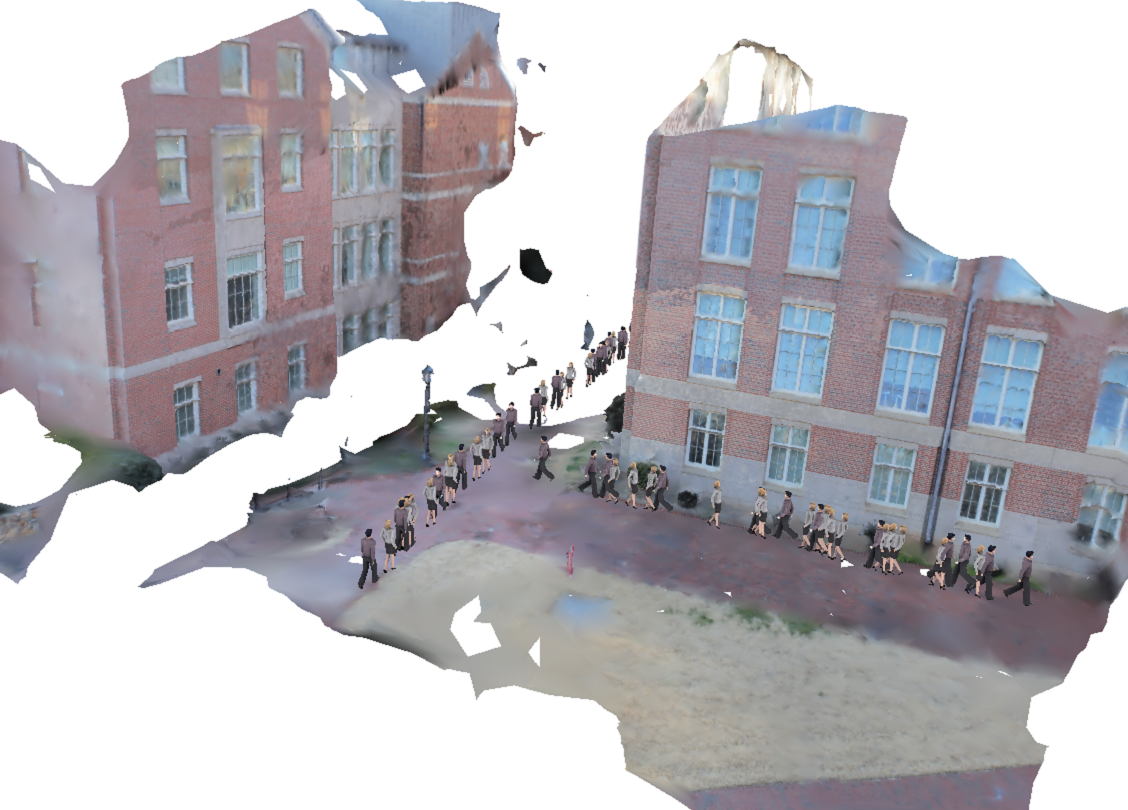
\includegraphics[height=0.18\textheight]{chapter4/resource/tjunction2.PNG}
}
\caption{Two views for each of the reconstructed results.}
\label{fig:reconstructed}
\end{figure}

\textbf{Synthetic datasets} Our first experiment uses synthetic data, with six different \oct~shapes on a plane, including a single line path, a T-junction path, a path with two parallel lines, a half circle path, sine wave shaped path, and two crossed path. For each of these shapes, we tested 32 instances, with each containing 50 randomly chosen object observation at different 3D positions. For more convenient error estimation during the evaluation, we normalized the 3D points so that the average distance between every pair of nearest points equals 1. The cameras are randomly generated around the 3D object points with two different configurations. In camera configuration A, all the camera centers stay in the same plane as the 3D points, which is more difficult since each viewing ray may intersect the ground truth path several times. In camera configuration B, the camera centers are set randomly off the plane, with the angle between the viewing ray and the plane being at most $10^\circ$ and camera distance of 2-3 times the length of the path. We choose $k=100$ uniformly distributed discrete 3D hypotheses $\mathbf{X}_i^o$  along each viewing ray $\mathbf{X}_i$ in a range that contains the ground truth 3D point. The size of the range is set as 1.5 times the length of the path. Notice that while the ground truth 3D points lie in the range, it is not guaranteed to be one of the discrete samples $\mathbf{X}_i^o$. %The run time of tGMST algorithm is set 1 hour for each data instance.

Errors are measured using the Euclidean distance between the estimated 3D points and the ground truth. The average errors over the 32 instances for each shape category are listed in Table \ref{fig:syntheticDataResult}. We report errors of the GMST output, and the errors after the continuous refinement using Eq. (\ref{equ:costFunc_continuous}).  Table \ref{fig:syntheticDataResult} shows our  continuous refinement always improves the reconstruction accuracy over the GMST approximation.  The results demonstrate    {\it off-plane} cameras yield improved results than {\it in-plane}  cameras  for  complex paths (e.g. crossed paths), due to the multiplicity of ray-to-path intersections. In these cases the GMST solution has a more complex search space and yields a sub-optimal solution. However, the condition number of the linear system does not vary significantly across configurations. Figure \ref{fig:synthetic} shows the estimated 3D points overlaid onto the ground truth.


\textbf{Real datasets} We evaluated our method on two image datasets  registered by VisualSFM \cite{WuVSFM}. The detection confidence threshold  is set high in order to lower down the false alarm rate. However, a very small amount of false alarms are purged manually as it may affect the reconstruction.  We sample 100 samples along the viewing ray in the range $[0,far]$, where $far$ is  estimated using the model scale. The running time for each object class trajectory is set to 3 hours.

The first dataset captures random pedestrians walking on the sidewalk, and random cars running on a lane. It contains 135 images with 82 valid car detections and 137 valid pedestrian detections. The scene and the reconstructed object class trajectory are shown in Figure \ref{fig:franklin_Recon}. %and the images are taken on the other side of the street at different time.
The second dataset captures several people who are walking on a T-junction shaped path at the corner of a building. It contains 47 images with 66 valid detections. Using the camera positions, we convert the face directions into the global coordinate system to obtain the motion tangents $\mathbf d_i$ of the moving people. For illustration, we construct the background static scene using CMPMVS \cite{JAN}. The general 3D human and car mesh models are inserted into each of the estimated 3D positions. We show different views of the reconstructed results in Figure \ref{fig:reconstructed}.

% show some images, and the results from different views.
%\begin{figure}[t]
%\begin{center}
%\begin{tabular}{|c ||c |c |c| c| }
%\hline
%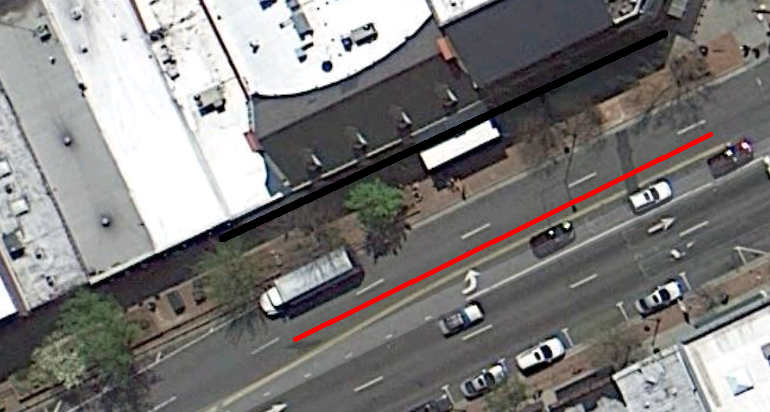
\includegraphics[width=0.192\textwidth]{chapter4/resource/googlescholar.PNG} &
%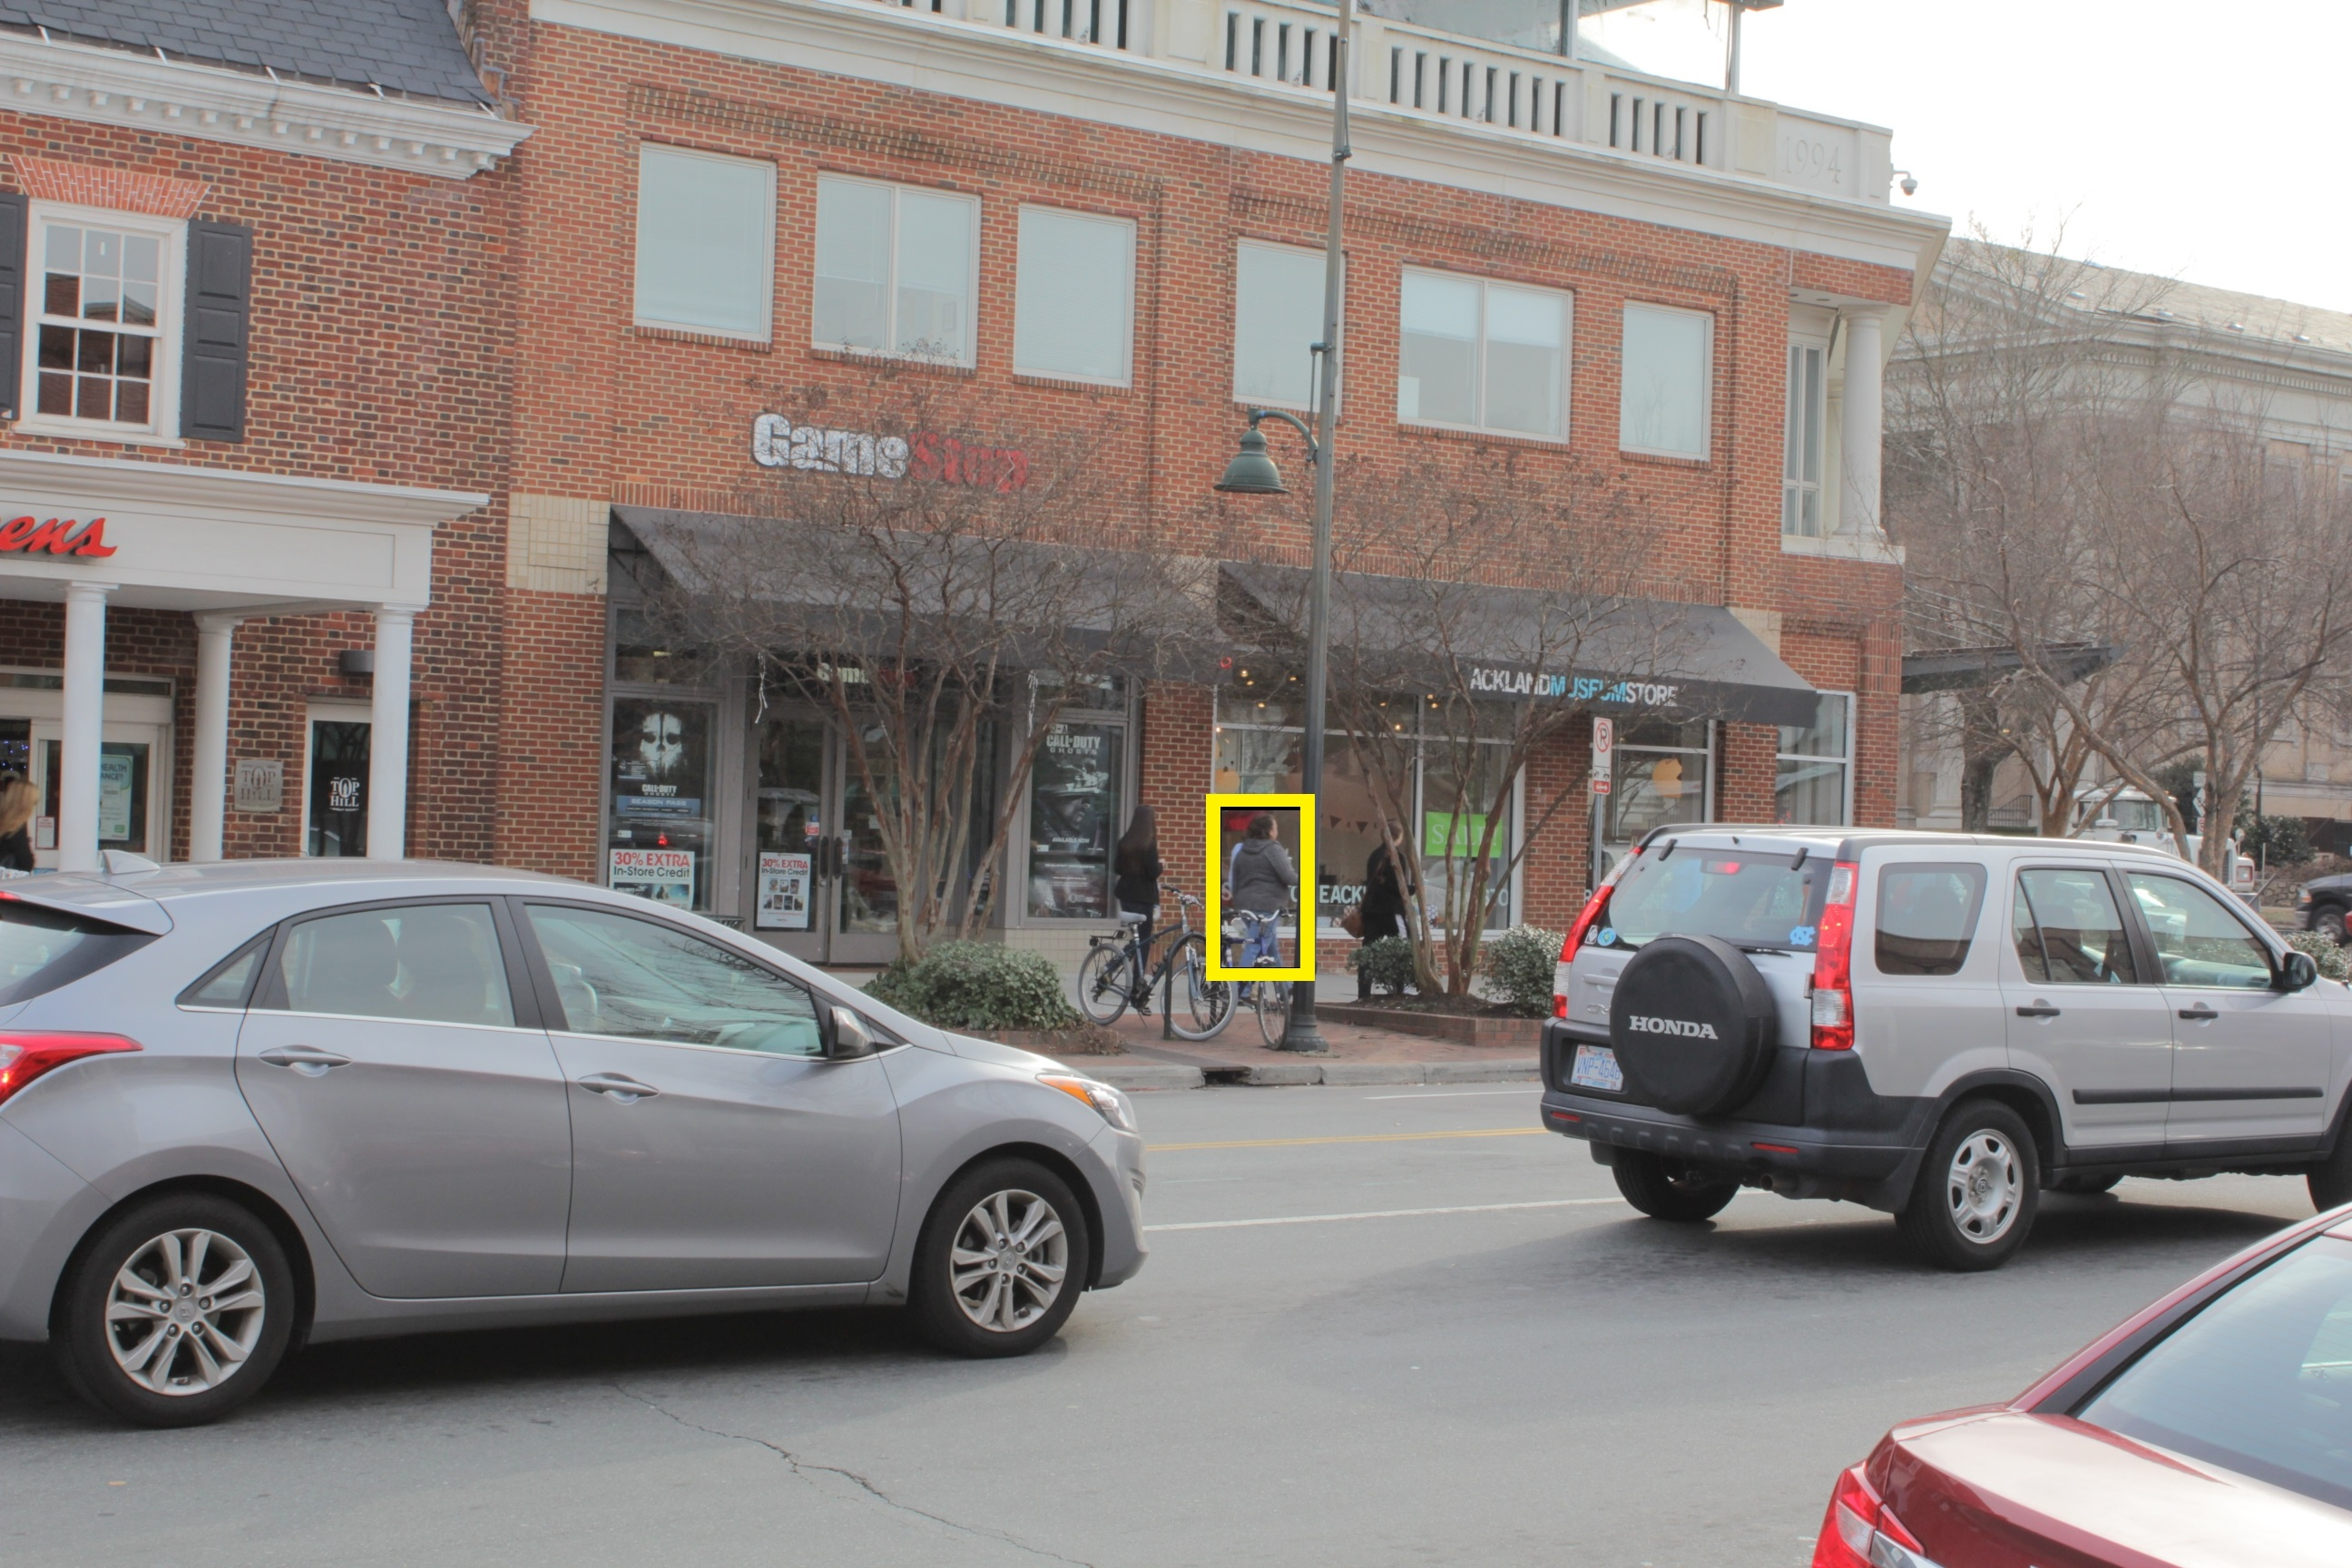
\includegraphics[width=0.192\textwidth]{chapter4/resource/cleanFrame083.jpg} & 
%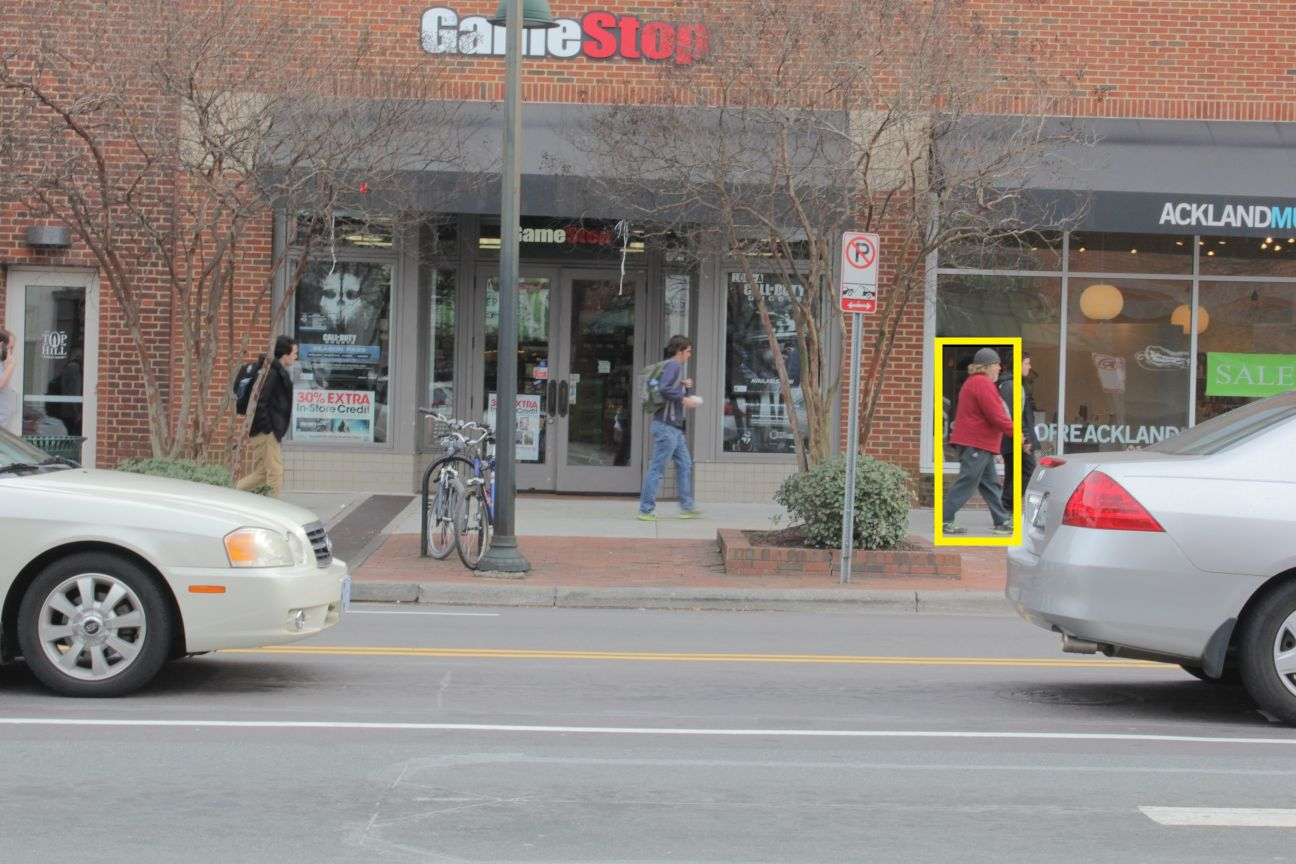
\includegraphics[width=0.192\textwidth]{chapter4/resource/cleanFrame084.jpg} & 
%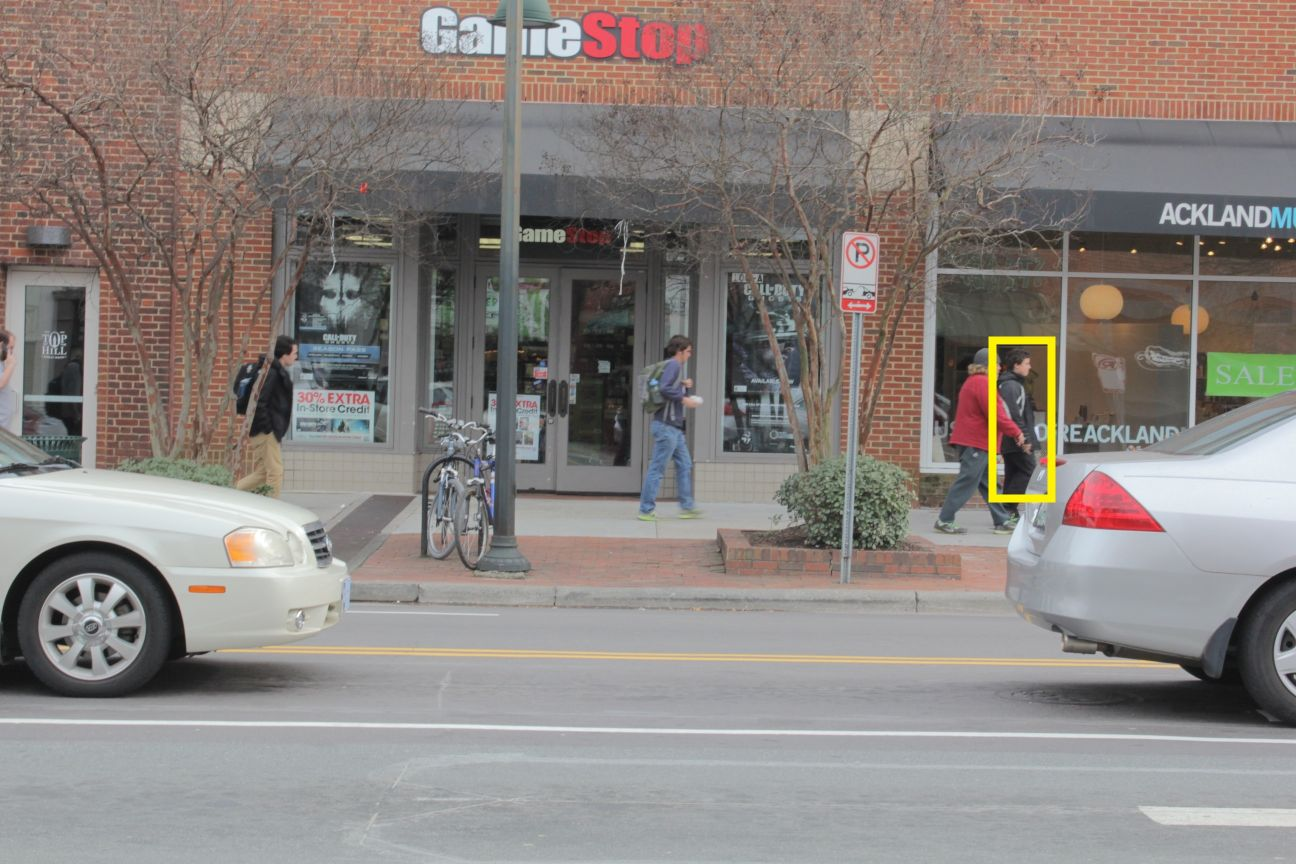
\includegraphics[width=0.192\textwidth]{chapter4/resource/cleanFrame085.jpg} &
%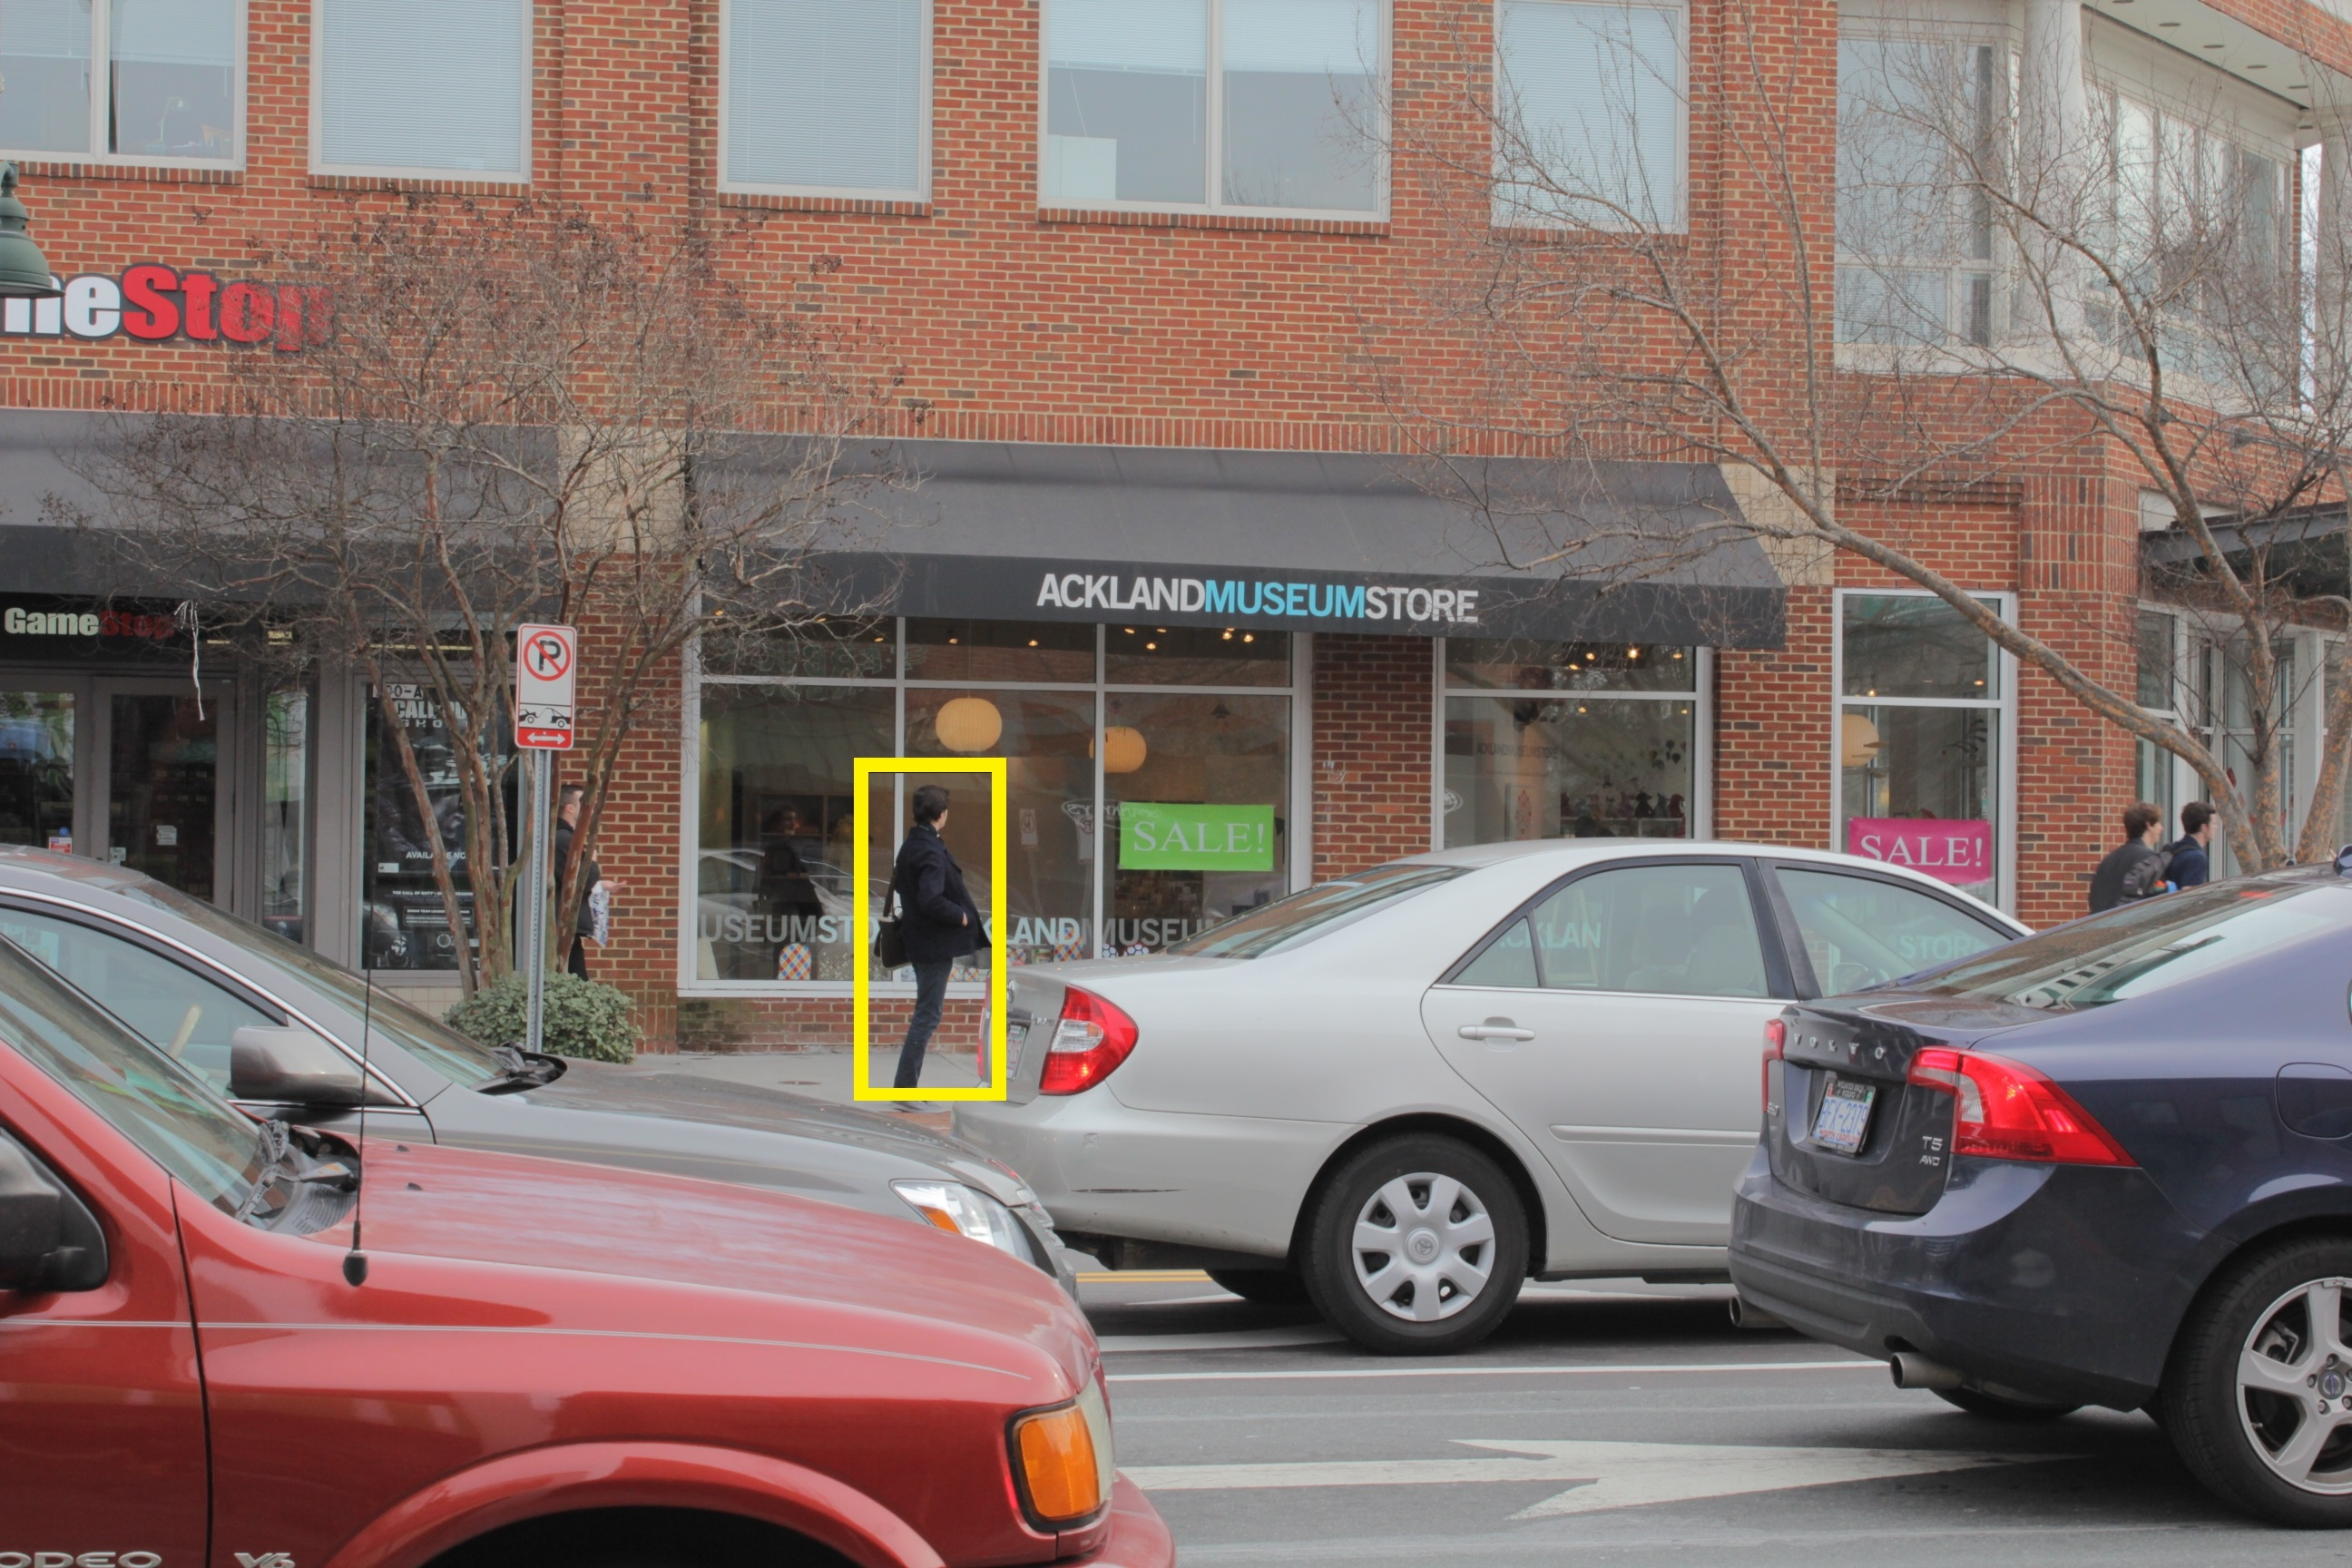
\includegraphics[width=0.192\textwidth]{chapter4/resource/cleanFrame086.jpg}\\
%\hline
%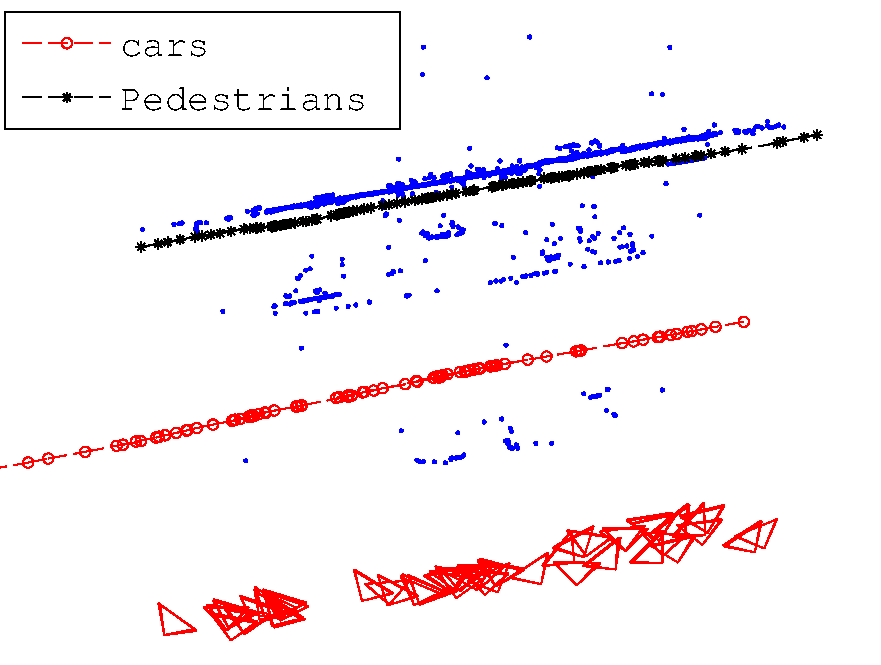
\includegraphics[width=0.192\textwidth]{chapter4/resource/car_ped_franklin_top.pdf} &
%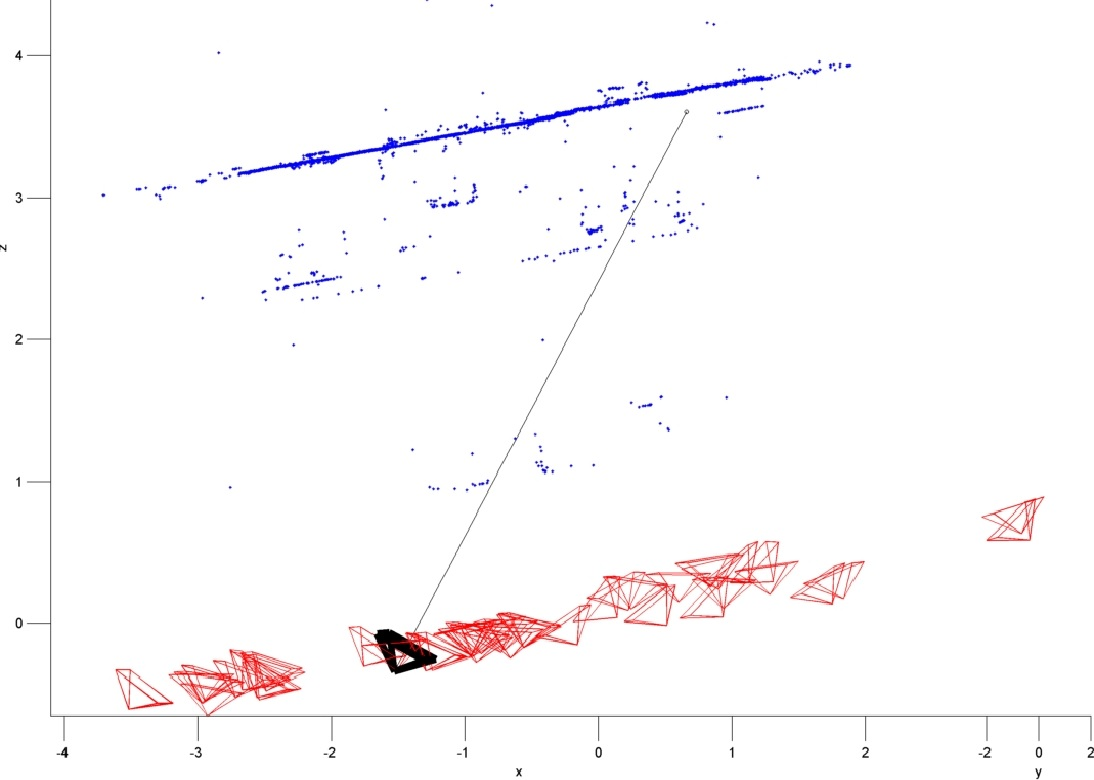
\includegraphics[width=0.192\textwidth]{chapter4/resource/Frame_083_crop.jpg} & 
%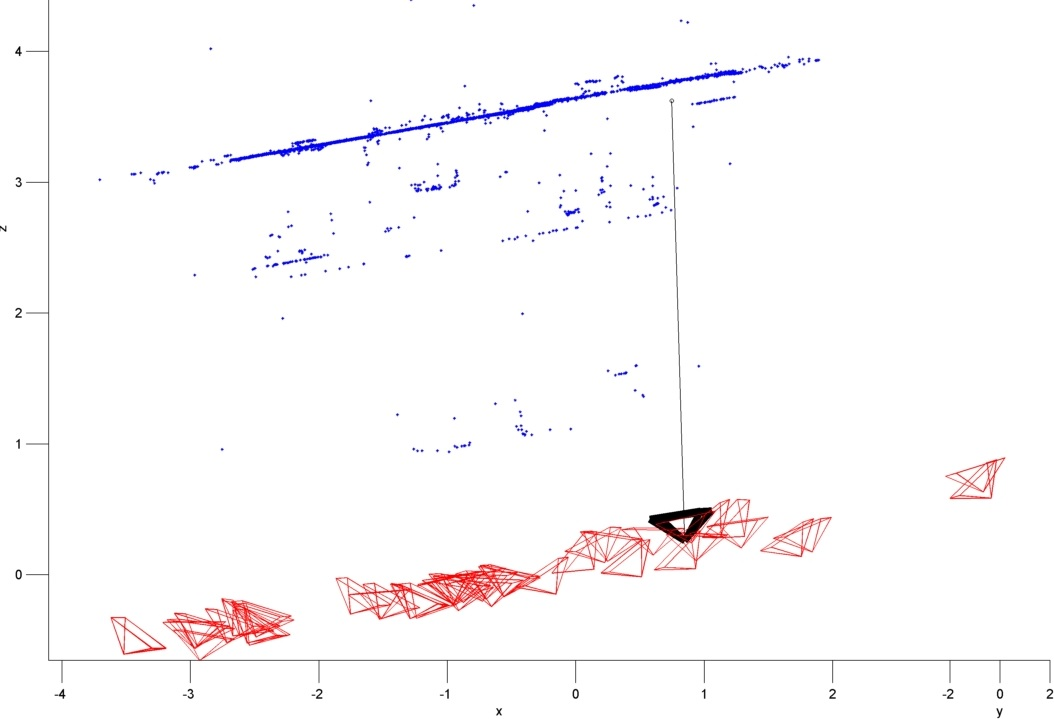
\includegraphics[width=0.192\textwidth]{chapter4/resource/Frame_084_crop.jpg} & 
%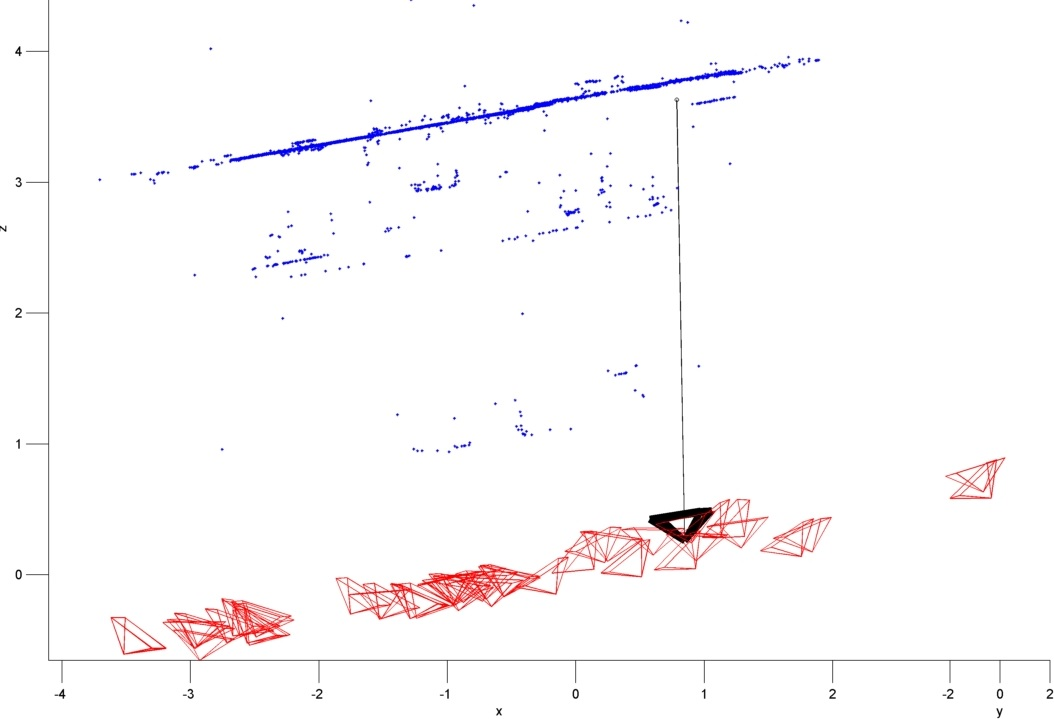
\includegraphics[width=0.192\textwidth]{chapter4/resource/Frame_085_crop.jpg} &
%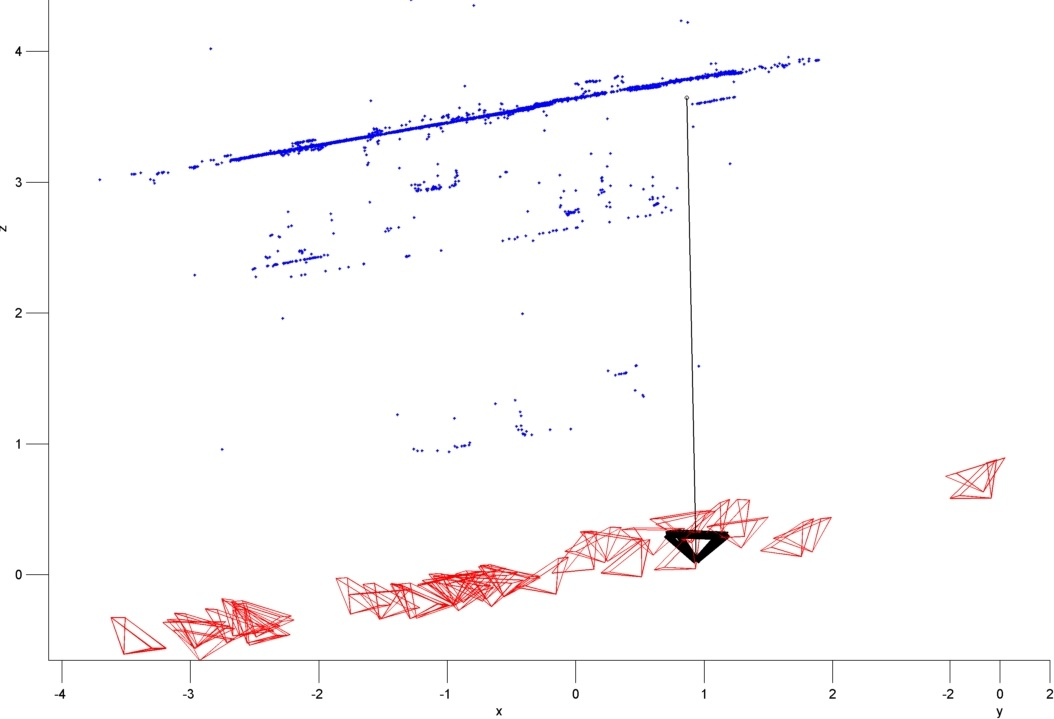
\includegraphics[width=0.192\textwidth]{chapter4/resource/Frame_086_crop.jpg}\\
%\hline
%\end{tabular}
%\end{center}
%\caption{The left column: an aerial image showing the scene and a figure showing the cameras and reconstructed cars and pedestrians. The right four columns: four pedestrian detections (shown in yellow rectangles) and the poses of the corresponding cameras. These four pedestrians are adjacent in the reconstructed object class trajectory. Notice that the second and the third images are the same image but with different detections.}
%\label{fig:franklin_Recon}
%\end{figure}

\begin{figure}[t]
\centering
\begin{tabu}{ |[2pt]c |[2pt] c |[2pt]}
\tabucline[2pt]{-}
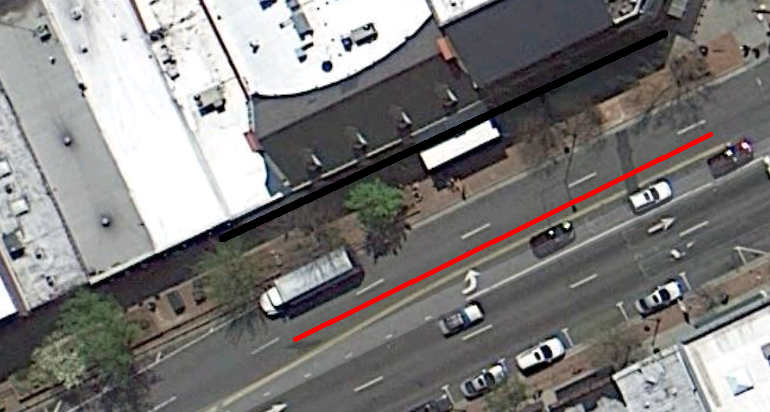
\includegraphics[width=0.33\textwidth]{chapter4/resource/googlescholar.PNG} &
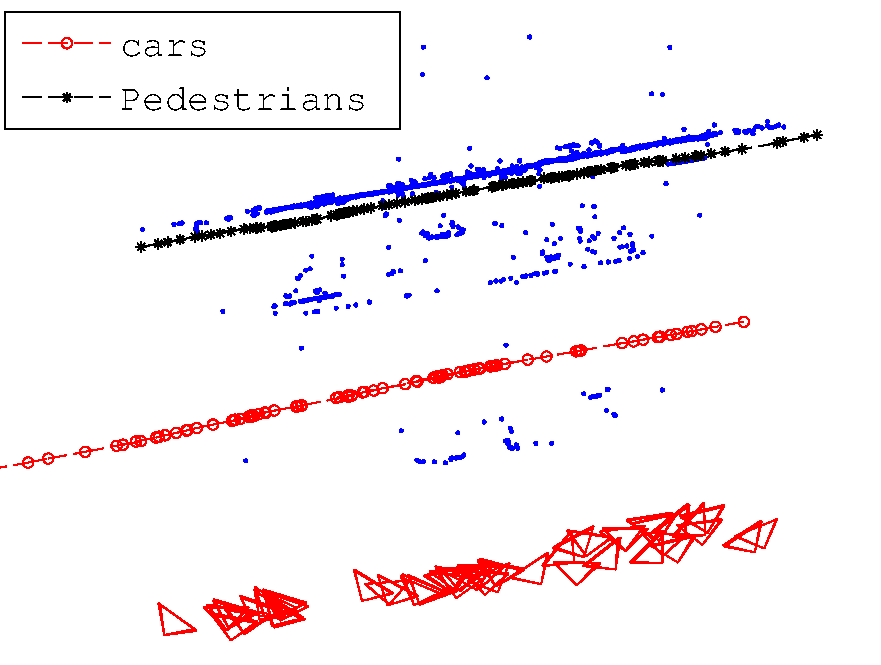
\includegraphics[width=0.33\textwidth]{chapter4/resource/car_ped_franklin_top.pdf}  \\
\tabucline[2pt]{-}
\tabucline[2pt]{-}
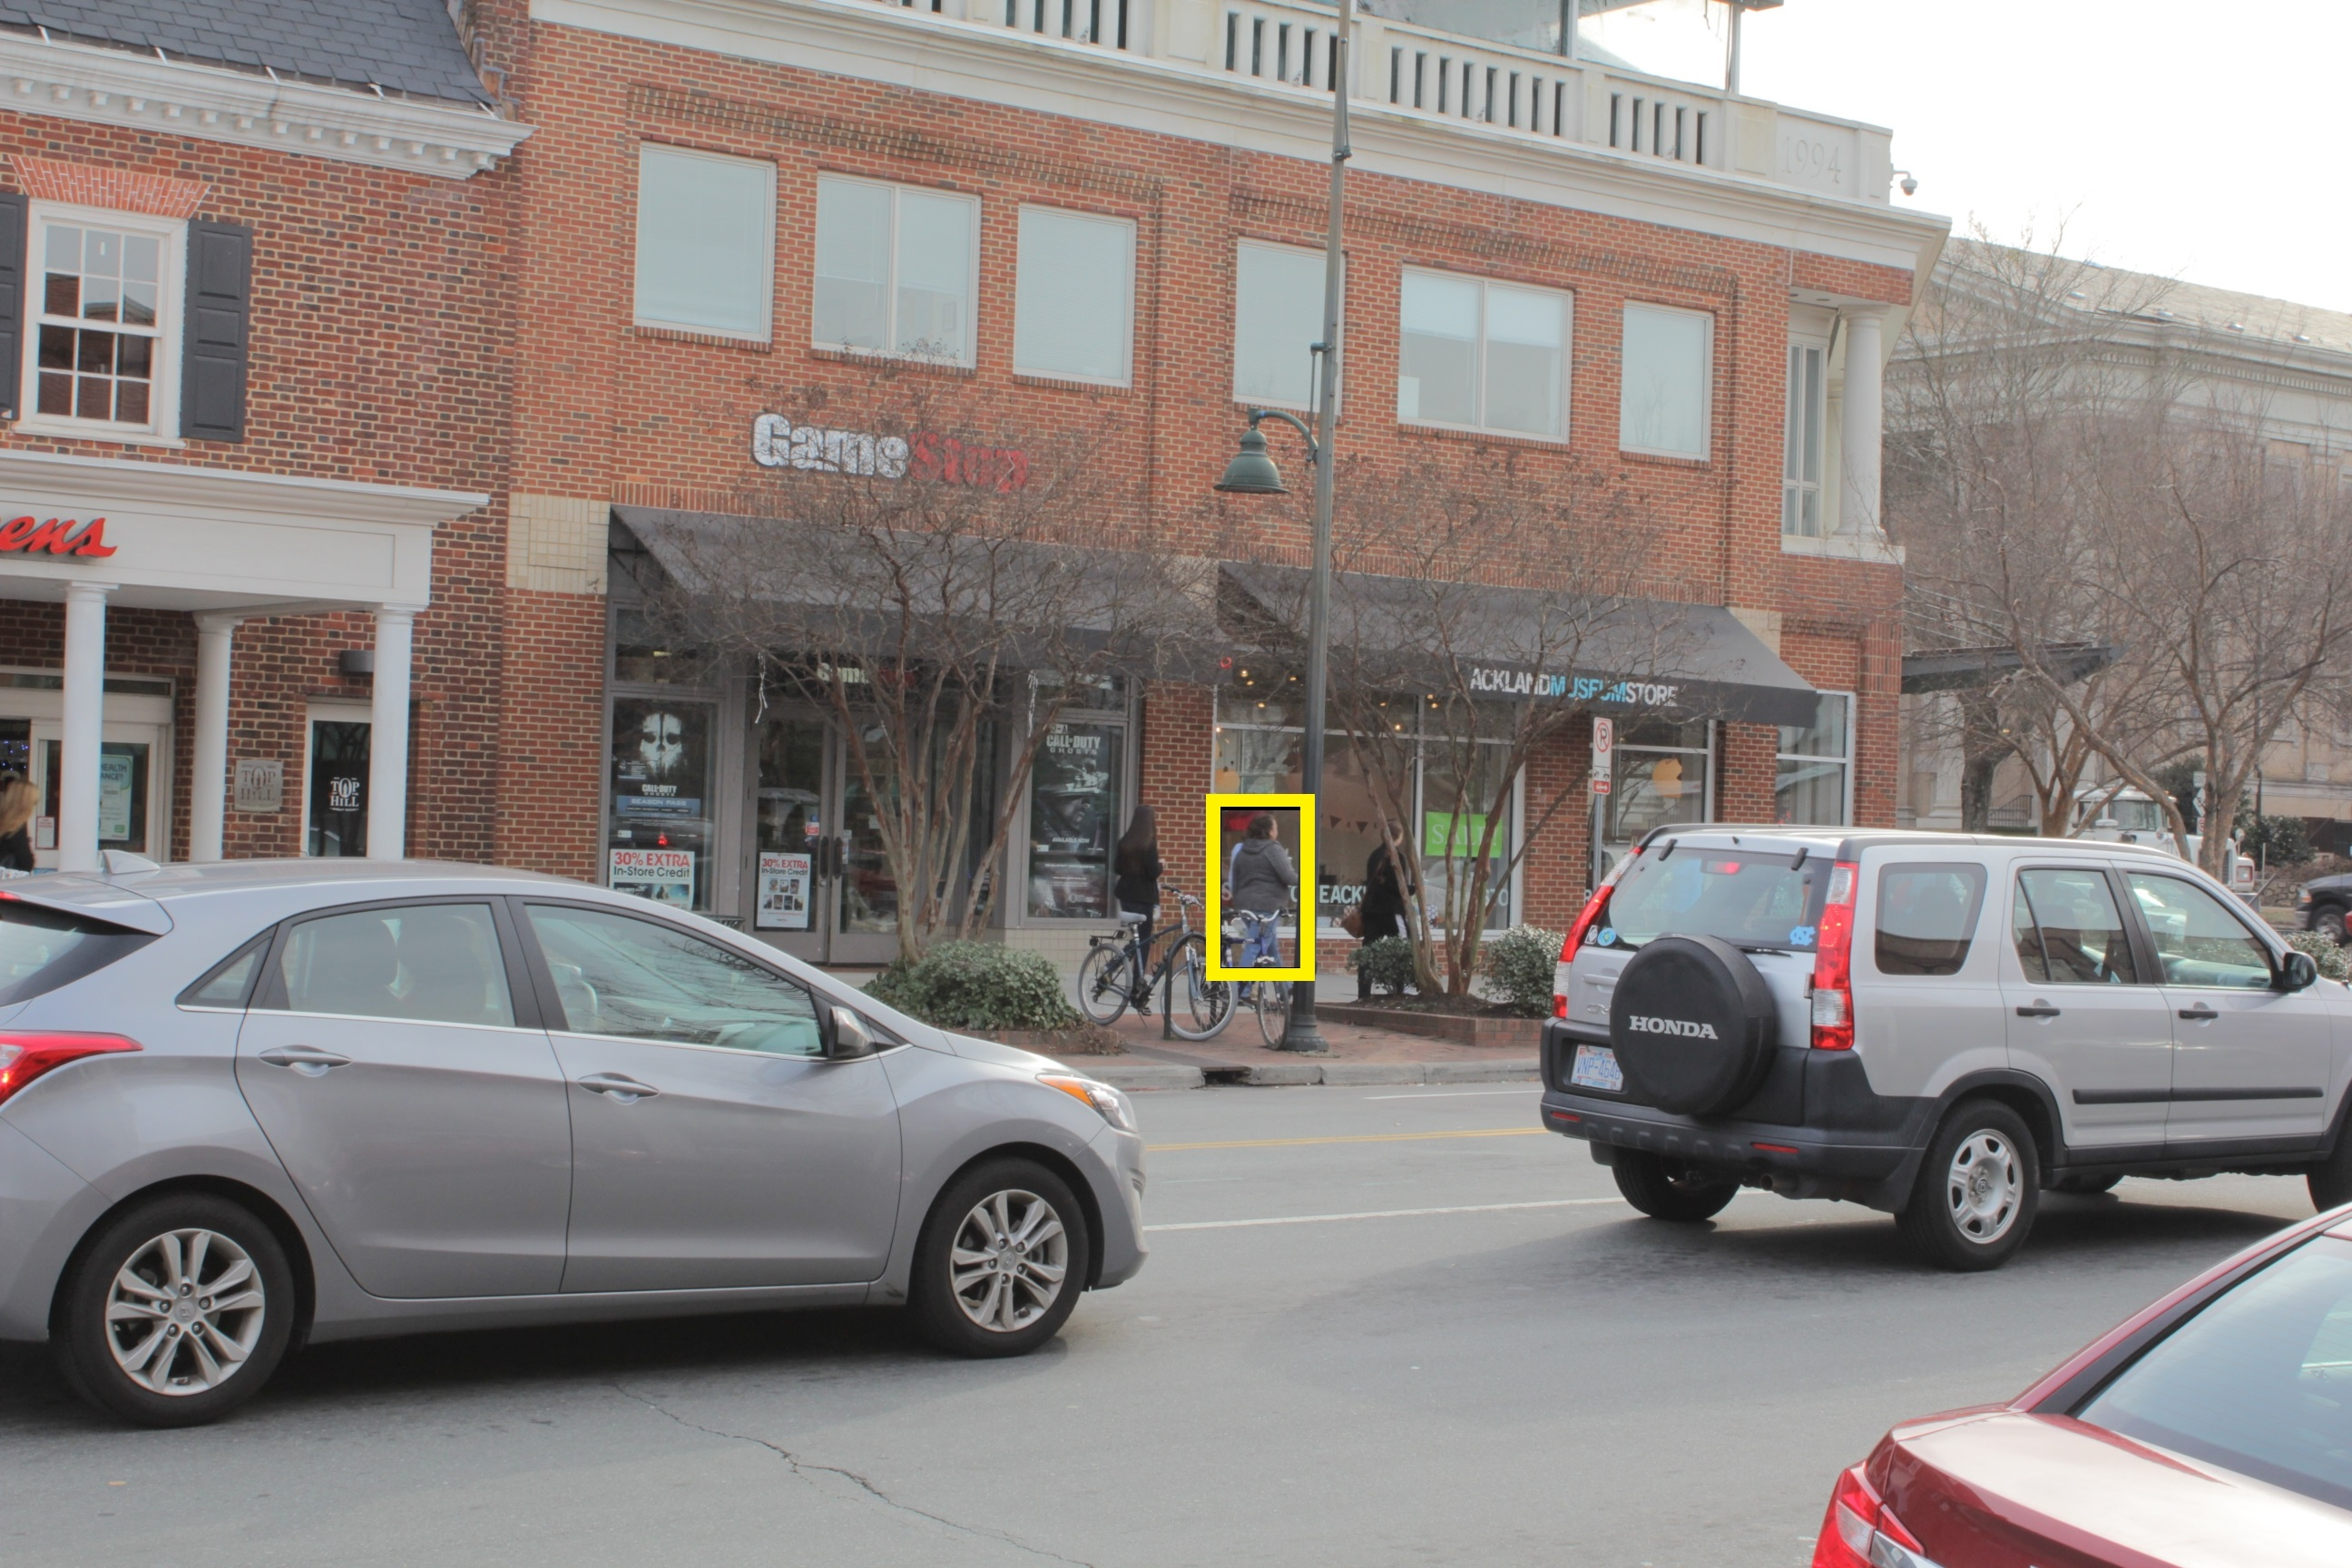
\includegraphics[width=0.33\textwidth]{chapter4/resource/cleanFrame083.jpg} & 
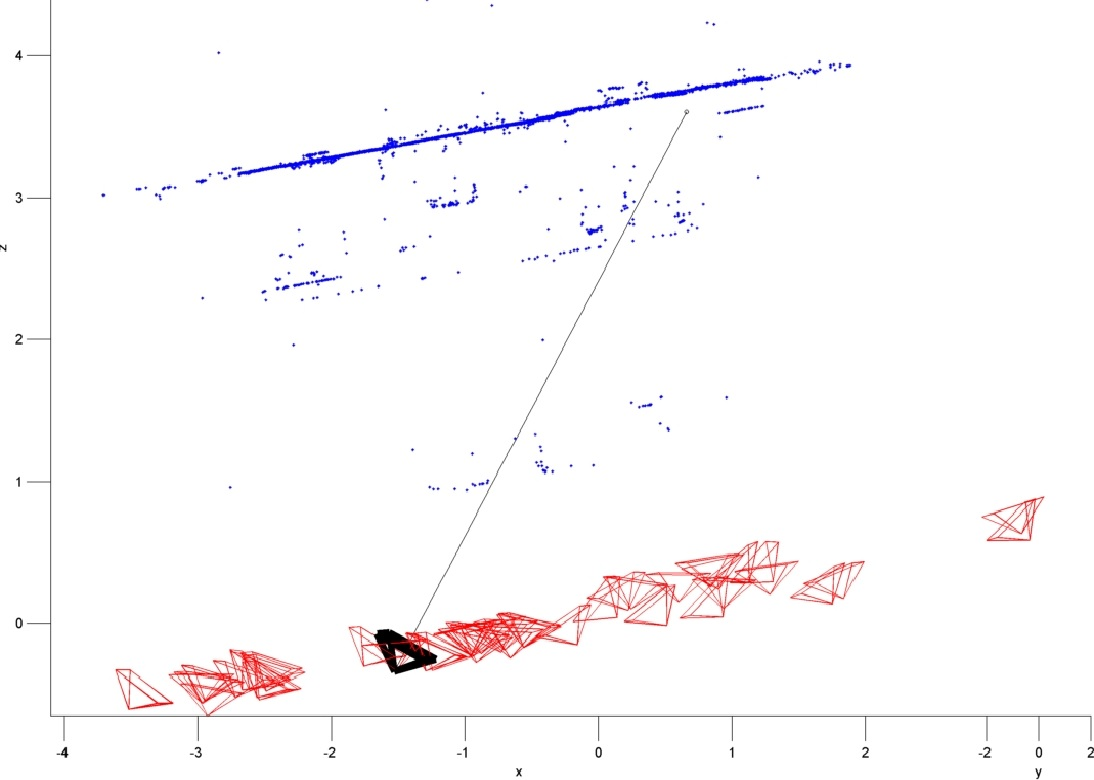
\includegraphics[width=0.33\textwidth]{chapter4/resource/Frame_083_crop.jpg}  \\
\tabucline[2pt]{-}
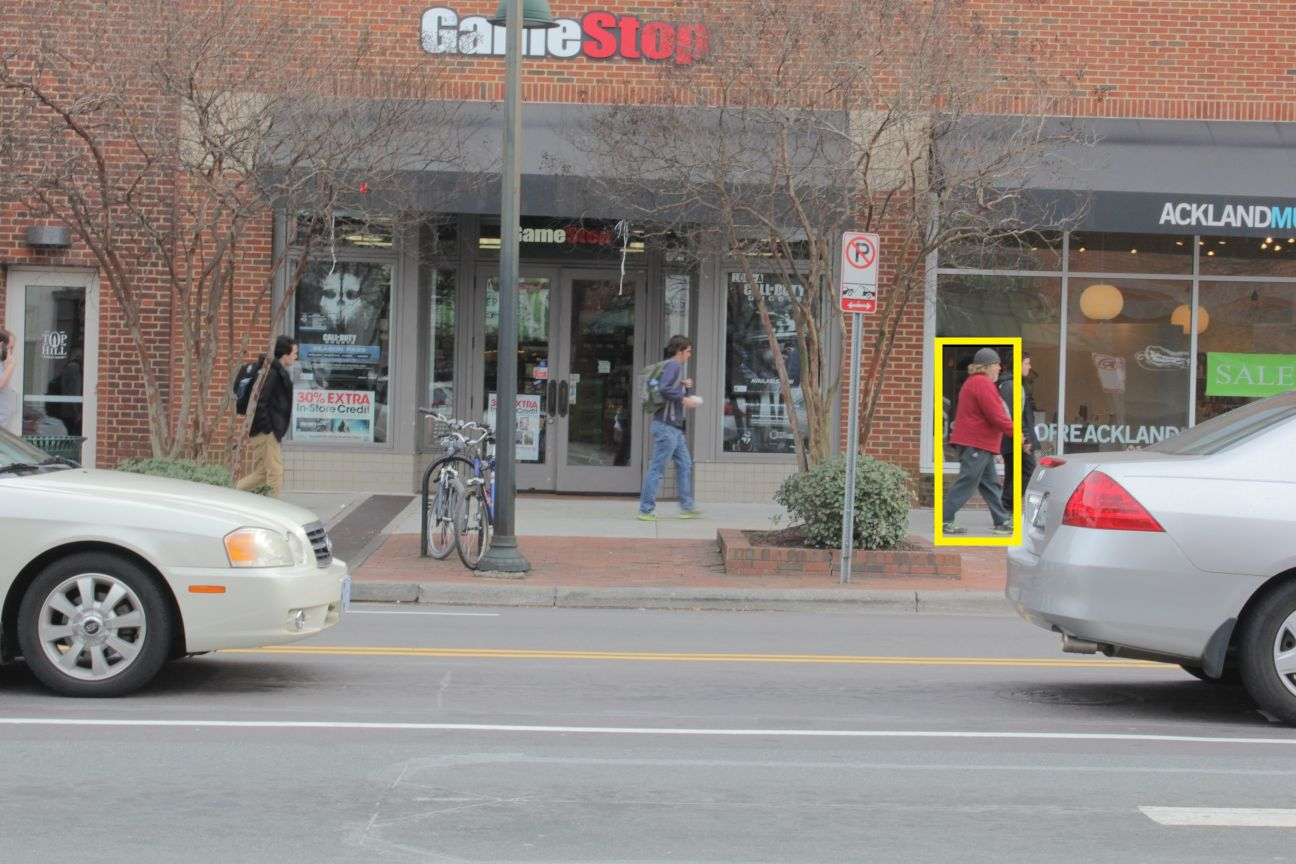
\includegraphics[width=0.33\textwidth]{chapter4/resource/cleanFrame084.jpg} &
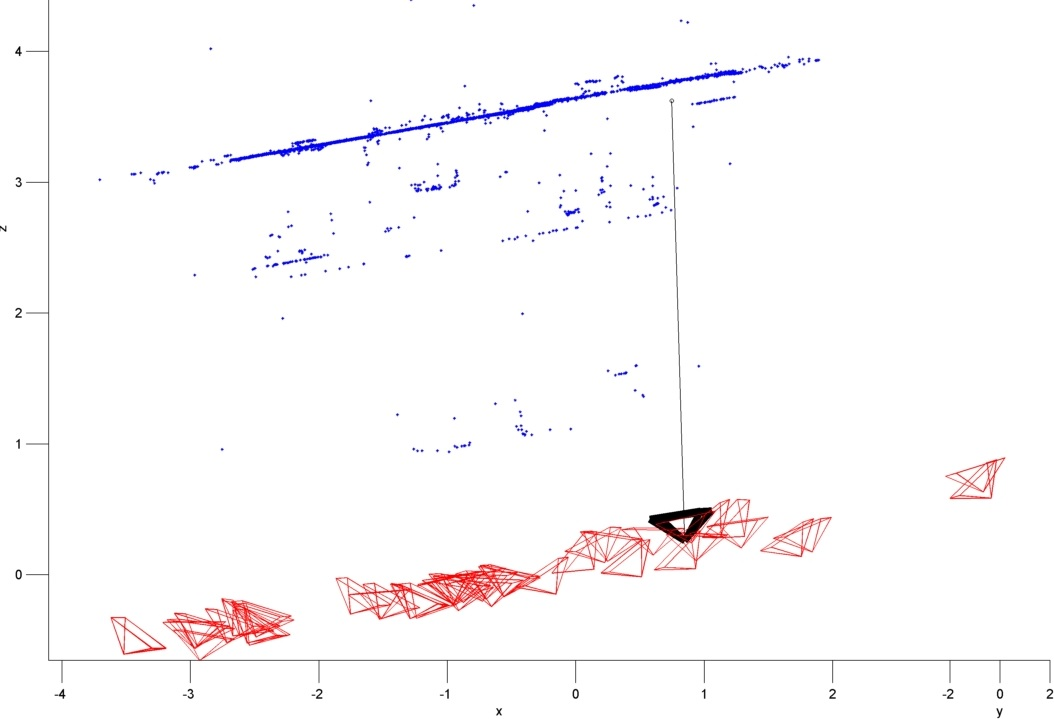
\includegraphics[width=0.33\textwidth]{chapter4/resource/Frame_084_crop.jpg} \\
\tabucline[2pt]{-}
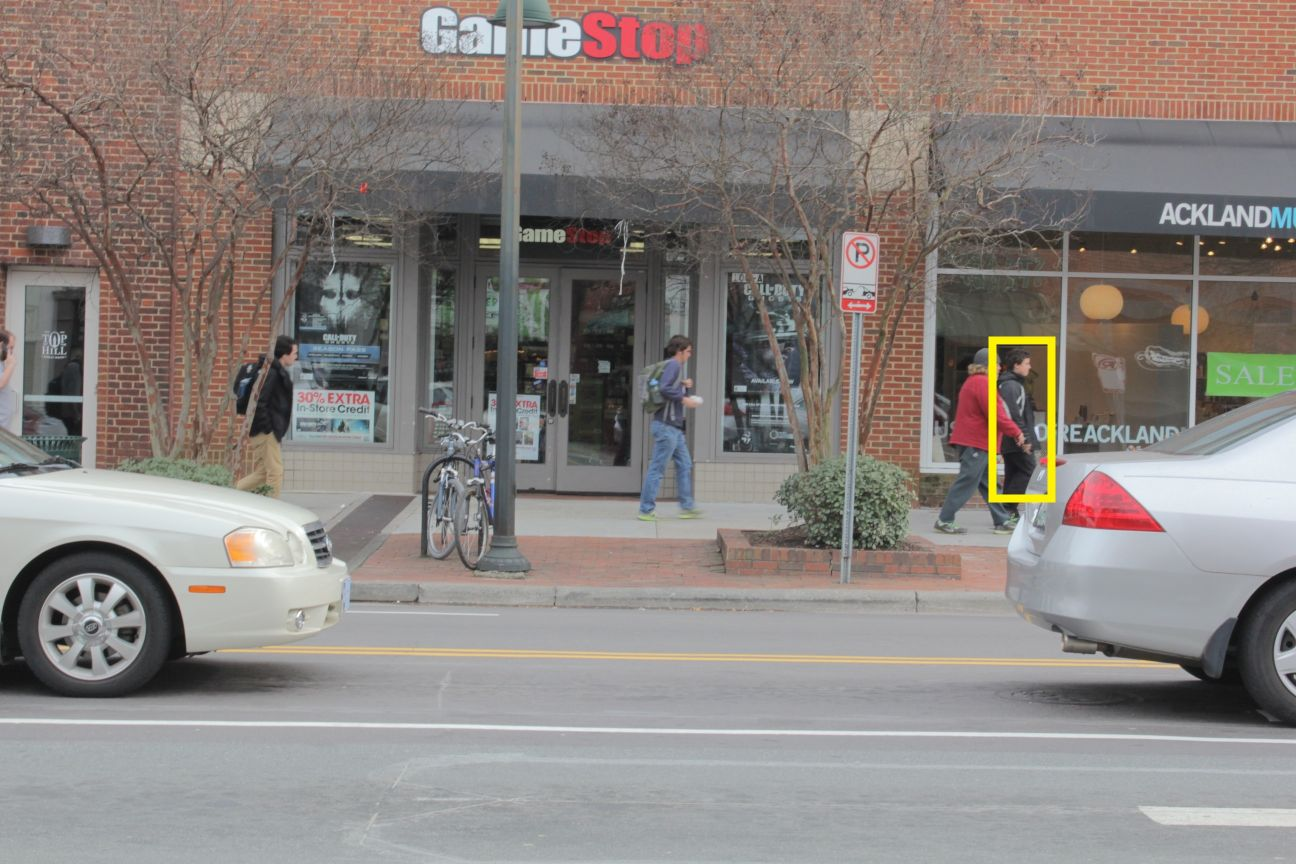
\includegraphics[width=0.33\textwidth]{chapter4/resource/cleanFrame085.jpg} & 
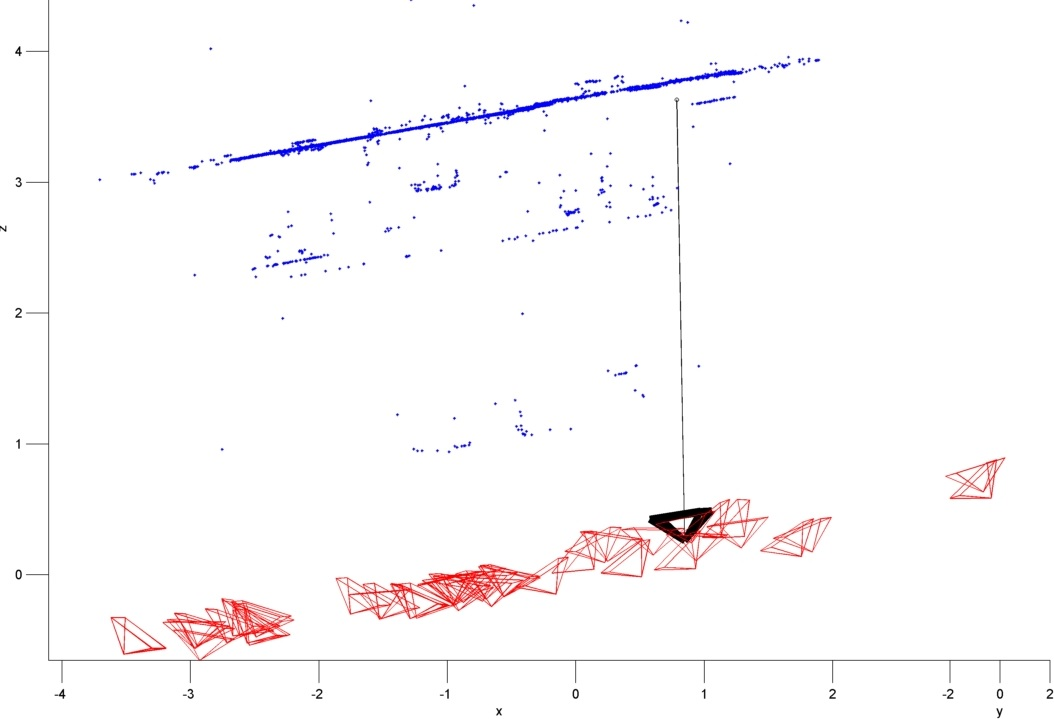
\includegraphics[width=0.33\textwidth]{chapter4/resource/Frame_085_crop.jpg} \\
\tabucline[2pt]{-}
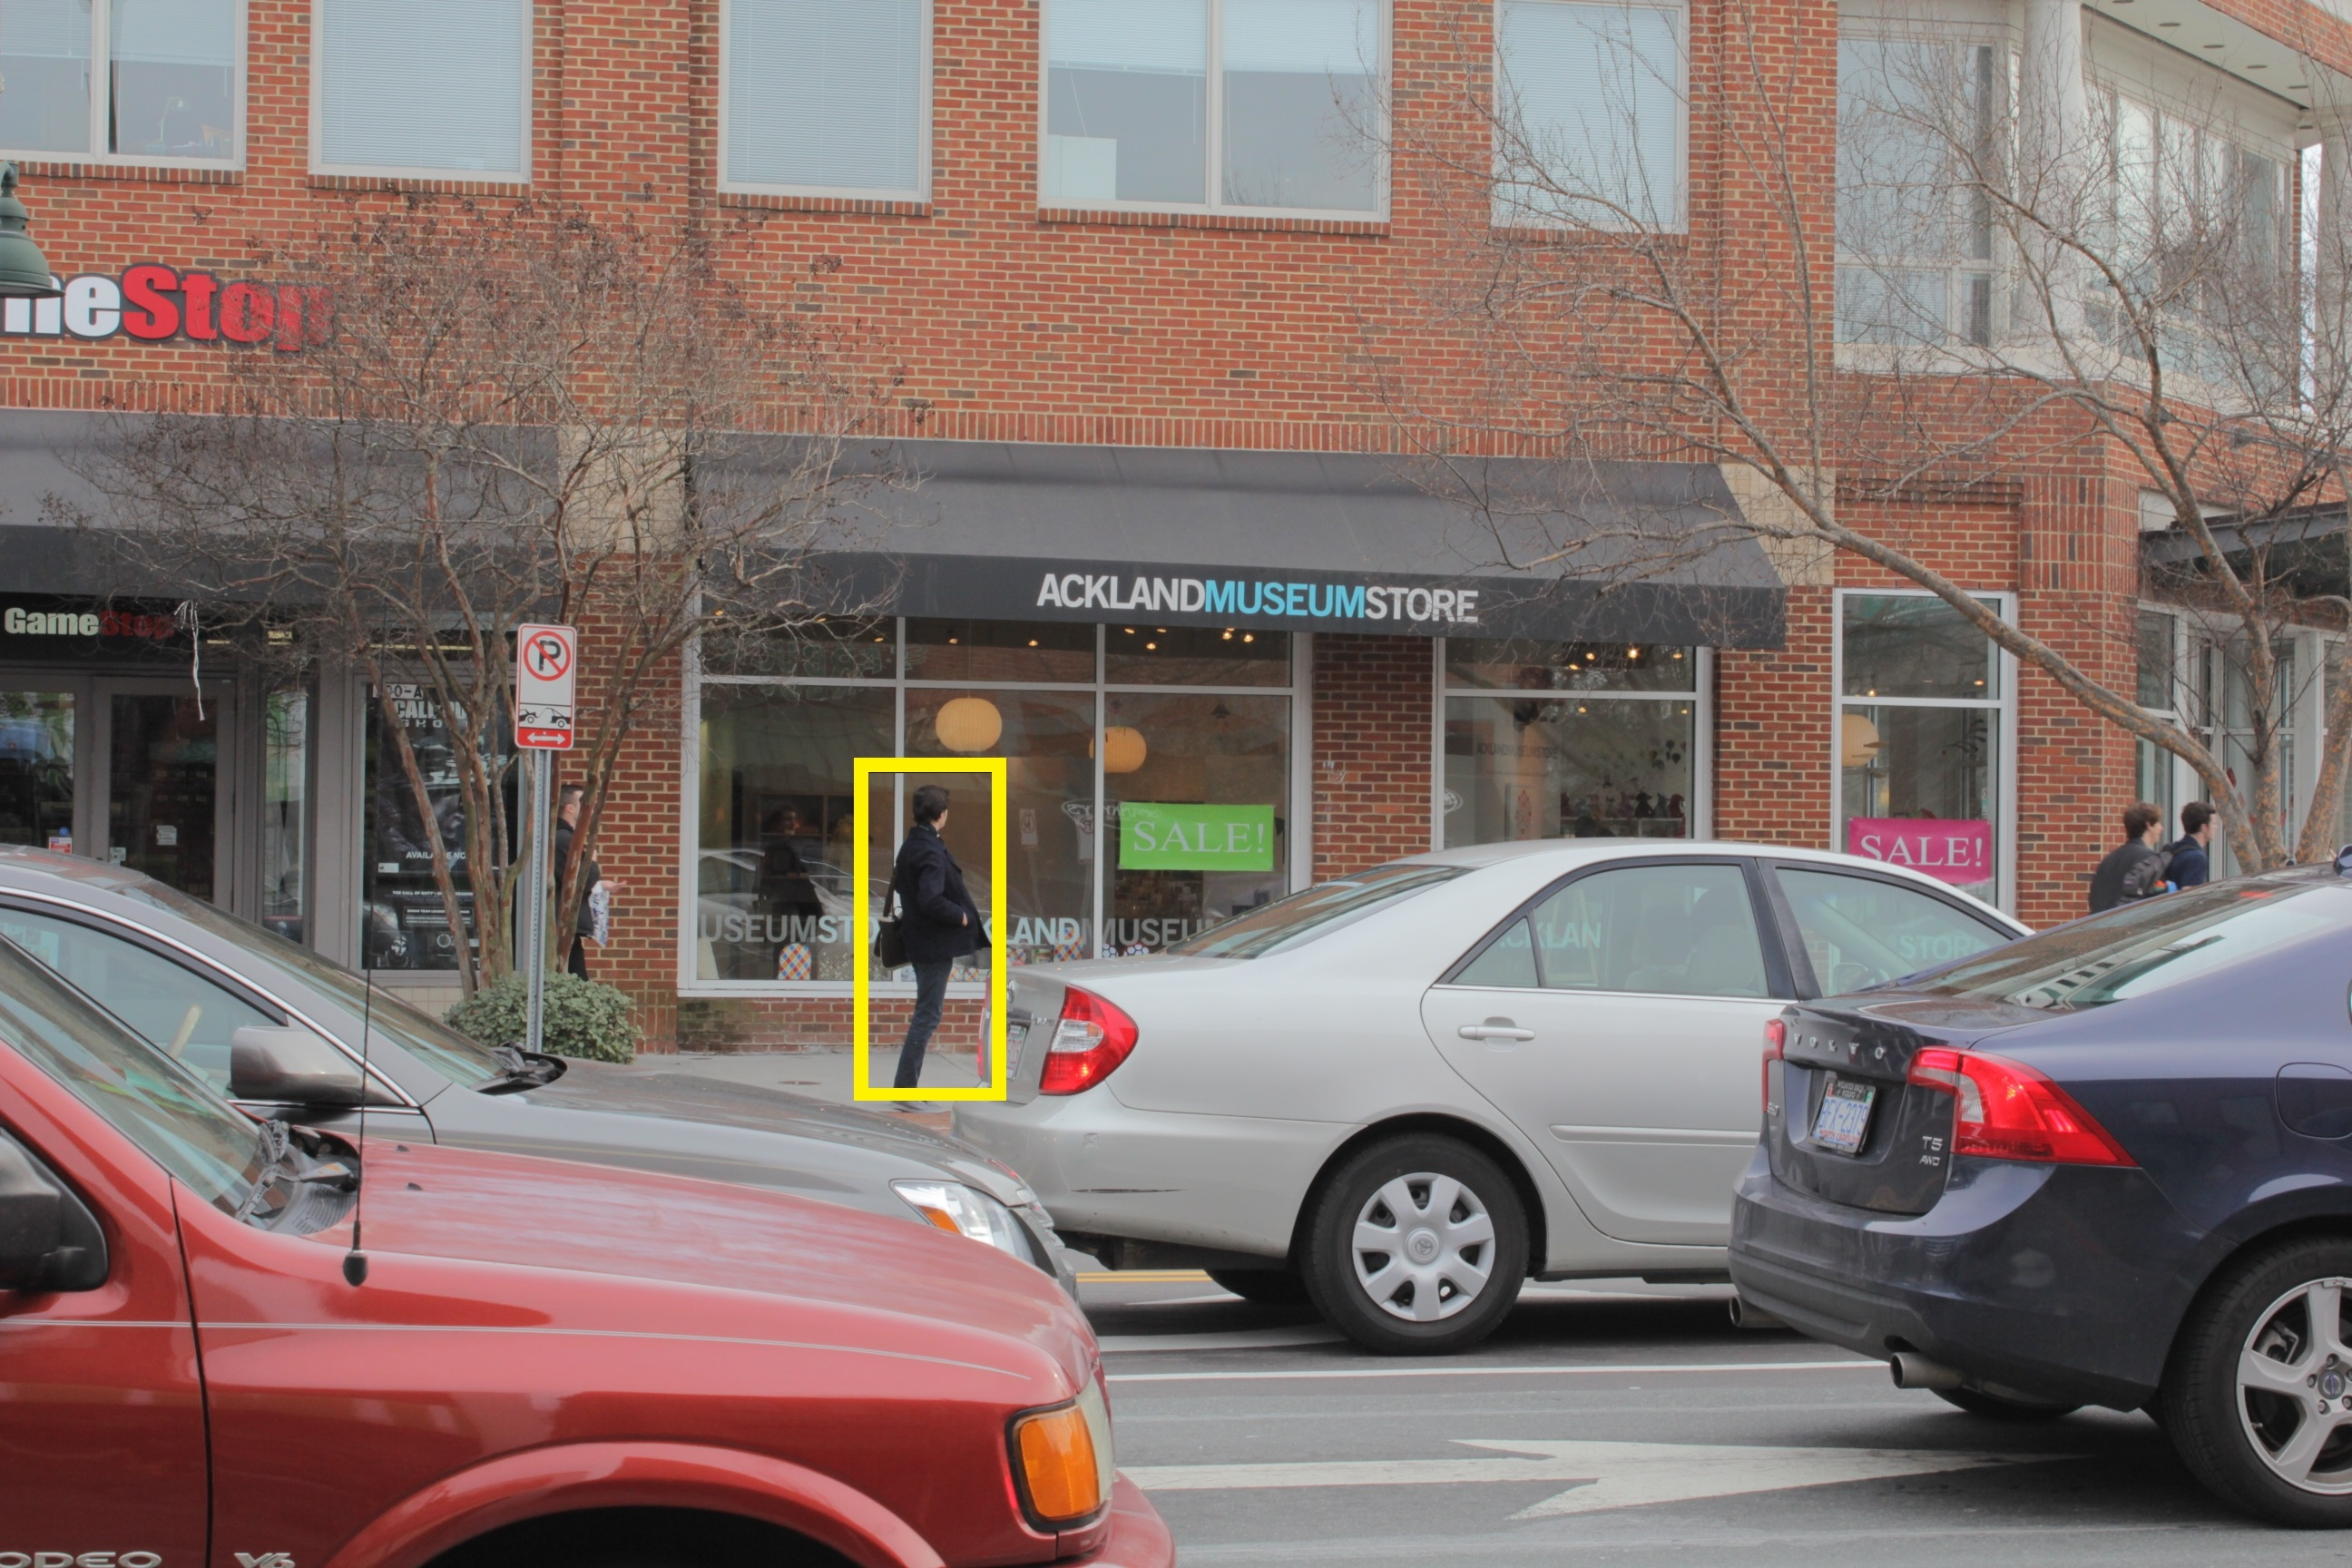
\includegraphics[width=0.33\textwidth]{chapter4/resource/cleanFrame086.jpg} &
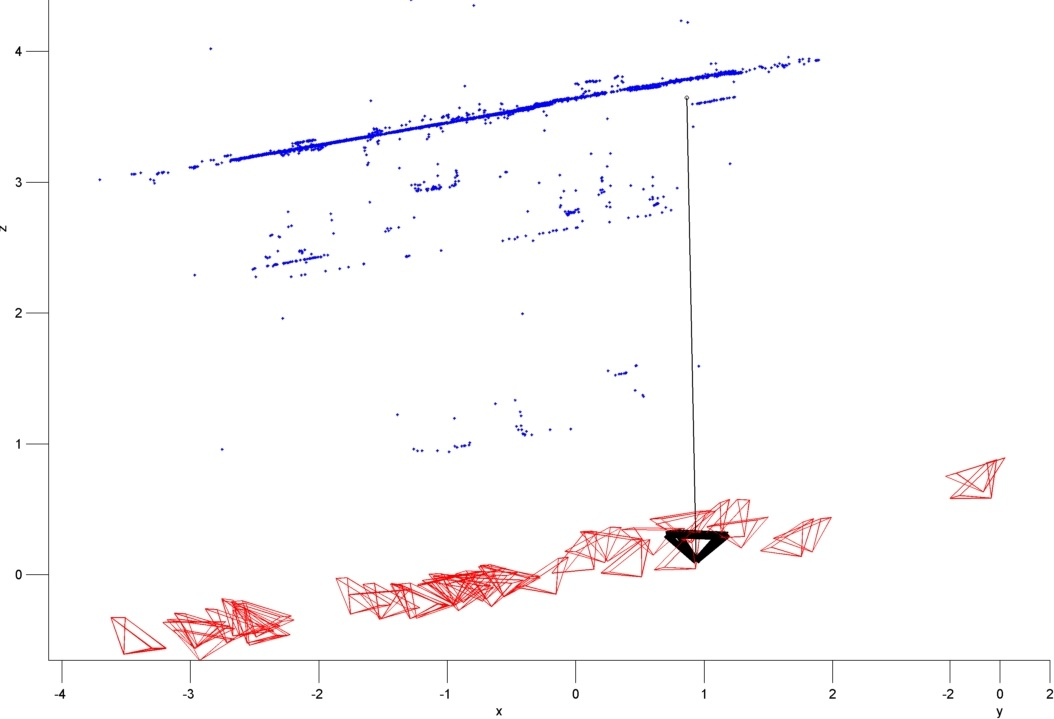
\includegraphics[width=0.33\textwidth]{chapter4/resource/Frame_086_crop.jpg}\\
\tabucline[2pt]{-}
\end{tabu}
\caption{The left row: an aerial image showing the scene and a figure showing the cameras and reconstructed cars and pedestrians. The bottom four rows: four pedestrian detections (shown in yellow rectangles) and the poses of the corresponding cameras. These four pedestrians are adjacent in the reconstructed object class trajectory. Notice that the second and the third images are the same image but with different detections.}
\label{fig:franklin_Recon}
\end{figure}

\section{Conclusions}
We proposed a solution to the novel \jost~problem, which allows the reconstruction of an \oct~from unordered images for which the capture times are unknown and there is no requirement of more than one view observing any object instance. This problem has previously been seen as highly limited in reconstructabililty. We evaluated our proposed method on synthetic and real world datasets and show promising results demonstrating the feasibility of the proposed approach to solve the \jost~problem and in fact the first time demonstrating its solvability.

